\documentclass[11pt, a4paper, twoside, italian]{report}

\usepackage[italian]{babel}
\usepackage[utf8]{inputenc}

\usepackage{amsmath}
\usepackage{amsfonts}
\usepackage{amssymb}
\usepackage{amsthm}
\usepackage{titlesec}
\usepackage{multicol}
\usepackage{lettrine}

\usepackage{booktabs}
\usepackage{fancyhdr}
\usepackage{listings}
\setcounter{tocdepth}{4}
\usepackage{stmaryrd}
\usepackage[strict]{changepage}
\usepackage{libertine}
\usepackage{textcomp}
\usepackage{float}
\usepackage{multicol}
\usepackage{makecell}
\usepackage{stmaryrd}
\usepackage{amssymb}
\usepackage{caption}

\usepackage[margin=0.5in]{geometry}

\usepackage{hyperref}
\usepackage[capitalise]{cleveref}

\usepackage{graphicx}


\theoremstyle{plain}
\newtheorem{thm}{Teorema}
\newtheorem{cor}[thm]{Corollario}



\title{\textbf{\textit{\underline{Sicurezza delle Reti}}}}
\author{\textit{Marco Colognese}}
\date{\small Ottobre 2018}
\normalsize

\begin{document}
\maketitle
\tableofcontents
\newpage



\chapter*{Introduzione}
\addcontentsline{toc}{chapter}{Introduzione}
I sistemi (oggetti matematici) vengono costruiti con metodi formali basati su matematica e logica, migliorandone la loro \textbf{sicurezza}. La nostra \textit{information society} è caratterizzata dall'espansione di internet nel quale convergono le informazioni e comunicazioni. Le infrastrutture si basano quasi tutte su sistemi informativi connessi alla rete.\\
La sicurezza è un ambito interdisciplinare e conferisce potere ad un'organizzazione.


\section*{Sicurezza Informatica}
\addcontentsline{toc}{section}{Sicurezza Informatica}
\begin{itemize}
	\item \textit{\textbf{Computer Security}}: ha a che fare con la prevenzione e la scoperta di azione non autorizzate da utenti per mezzo di un sistema di computer. Si basa principalmente sul concetto di \textit{autorizzazione} e \textit{security policy}.
	\item \textit{\textbf{Network Security}}: si basa su un'infrastruttura di rete e politiche adottate dal suo amministratore. Si vuole proteggere la rete e le sue risorse da accessi non autorizzati.
	\item \textit{\textbf{Information Security}}: riguarda le informazioni, ricavabili dai dati, indipendentemente dai computer. Si occupa di proteggere l'informazione e i sistemi informativi da accessi, usi, modifiche o distruzioni non autorizzate.
	\item \textbf{Security policy}: indica che quali comportamenti del sistema sono ammessi o meno. Viene formulata per raggiungere delle \textit{security properties} (oppure \textit{security goals}) come la più nota \textbf{CIA}:
	\begin{itemize}
		\item \textbf{\textit{Confidentiality (Secrecy)}}: evitare che l'informazione venga rivelata a terzi;
		\item \textbf{\textit{Integrity}}: evitare modifiche da parte di terzi;
		\item \textbf{\textit{Availability}}: evitare problemi di funzionalità/servizio (es. \textit{DoS attack}).
		\item \textit{Accountability}: per tenere traccia dei responsabili delle azioni tramite log che vengono poi spediti ad un altro server online per evitare che vengano corrotti quando il sistema viene attaccato;
		\item \textit{Authentication}: per verificare l'identità degli utenti, l'origine dei dati e permettere un \textit{access control}. Può essere effettuata con qualcosa che si ha (card), che si conosce (password) o che si è (firma, impronta digitale);
	\end{itemize}
	\item \textbf{Security mechanisms}: per far rispettare la policy del sistema (in tutti gli \textit{ambienti malevoli}).
\end{itemize}


\subsection*{Protezione di un Sistema}
\begin{itemize}
	\item \textit{Prevention}: si vogliono prevenire brecce del sistema con opportune tecnologie di sicurezza e difesa (es. firewall);
	\item \textit{Detection}: in caso di attacco, è necessario individualo attraverso \textit{intrusion detection systems} (es. file di log);
	\item \textit{Response}: in caso di breccia, è necessario avere dei metodi per il recupero degli assets attraverso dei backup e interpellando le forze dell'ordine.
	\newline
\end{itemize}

\begin{multicols}{2}
	~\\
	\noindent
	Quando si lavora per la sicurezza di un sistema, vanno prese contromisure per effettuare \textbf{risk minimization}, limitando il più possibile le vulnerabilità ad un valore accettabile, per mettere al sicuro gli assets da potenziali furti.
	\columnbreak
	\begin{figure}[H]
		\centering
		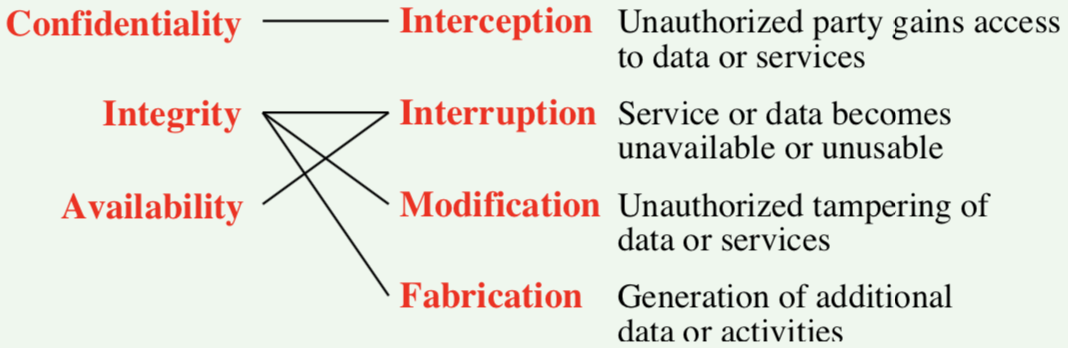
\includegraphics[scale=0.5]{threats}
	\end{figure}
\end{multicols}
\noindent
Una \textbf{vulnerabilità} è una debolezza del sistema che può essere sfruttata da un \textit{attacco} per creare un danno.\\
Esse emergono quando si ha a che fare con un ambiente ostile: pc in mani sbagliate, internet, software vari.\\

\noindent
L'\textbf{Analisi del Rischio} e la sua riduzione si divide in passi:
\begin{itemize}
	\item analisi dei rischi esistenti: identificare gli assets da proteggere e i rischi ai quali sono esposti;
	\item analisi delle soluzioni di sicurezza: quale contromisura riduce i rischi, valutando anche i rischi che porterà.
\end{itemize}

\noindent
Il \textbf{Managing Security} prevede alcuni passi per implementare una soluzione:
\begin{itemize}
	\item \textit{security analysis}: indaga sui possibili attacchi che possono mettere a rischio gli assets, proponendo una policy e soluzioni con un costo appropriato.
	\item \textit{threat model}: documenta i possibili attacchi ad un sistema, immaginando tutte le vulnerabilità sfruttabili.
	\item \textit{risk assessment}: studia la probabilità di un attacco nell'ambiente del sistema e gli assegna un costo (trova il rischio).
	\item \textit{security policy}: elenca i possibili attacchi e le rispettive contromisure possibili. Si analizzano i costi delle contromisure in relazione al rischio per ottenere un compromesso valido.
	\item \textit{security solution}: vengono distribuite le tecnologie appropriate al costo adeguato; è un lavoro di bilancio ma è giusto fare gli sforzi giusti dove necessario.
\end{itemize}


\subsection*{Formal Methods}
\begin{multicols}{2}
\noindent
Si costruisce un modello formale dei comportamenti del sistema (astrazione del programma concreto). Vengono formalizzati i requisiti come proprietà di sicurezza e si verifica che il sistema le soddisfi. Bisogna documentare come deve operare il sistema, i requisiti di sicurezza in modo non ambiguo e validare il sistema tenendo conto dei requisiti.
\columnbreak
\begin{figure}[H]
	\centering
	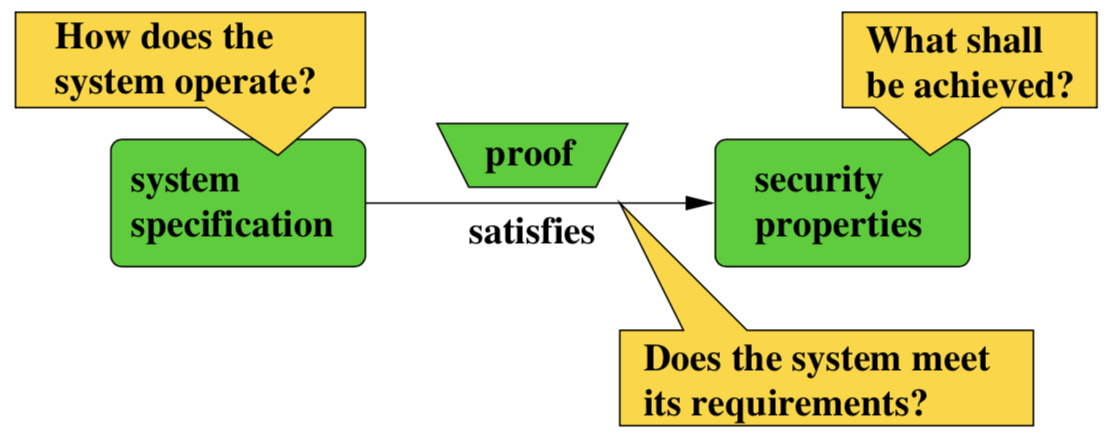
\includegraphics[scale=0.4]{formalmethods}
\end{figure}
\end{multicols}


\section*{Privacy in Network Security}
\addcontentsline{toc}{section}{Privacy in Network Security}
La \textit{confidenzialità} riguarda l'introduzione di un \textit{access control} per evitare che certe informazioni vengano lette da persone non autorizzate. Spesso con \textit{privacy} si intende l'\textit{anonimità}: mantenere privata l'identità.
\begin{itemize}
	\item \textit{Privacy}: scegliere cosa gli altri possono sapere (confidenzialità delle informazioni non si vogliono condividere).\\
	\textit{Data Protection}: assicurare che i nostri dati non siano distribuiti e usati in modi indesiderati (si segue una \textit{policy}).
	\item \textit{Anonimity}: condizione nella quale la vera identità non è conosciuta (confidenzialità della propria identità).\\
	\textit{Inosservabilità} delle azioni nel momento in cui vengono effettuate.
\end{itemize}
\noindent
L'\textit{\textbf{anonimità}} è difficile da ottenere in una rete pubblica poiché gli headers dei pacchetti identificano i destinatari e nella rete è possibile effettuare \textit{traffic analysis} (servono tecnologie per contrastarla).\\
Nonostante il payload sia criptato, è comunque visibile ed è possibile violare l'anonimità.
\\
\textit{\textbf{Anonimity Set}}: l'unico livello di anonimità in rete è dato dal fatto che le \textit{azioni} di una persona possono essere osservate ma \textit{non distinte} da quelle di altri. Questo gruppo è chiamato \textit{anonymity set} (più è grande, meglio è).\\
\\
L'obiettivo è rendere anonimi mittenti e destinatari durante le comunicazioni per dare confidenzialità alle identità.
\begin{itemize}
	\item \textit{ricevitore}: reso anonimo quando si spediscono messaggi in broadcast o multicast (nell'anonymity group).
	\item \textit{mittente}: i pacchetti (es. le richieste $HTTP$), vengono anonimizzate dai server proxy. Il \textbf{problema} è che il \textit{proxy} conosce tutto (si può fare \textit{traffic analysis}). Le \textbf{soluzioni} sono catene di proxy in cascata, \textit{mix networks} $\dots$
\end{itemize}
\begin{figure}[H]
	\centering
	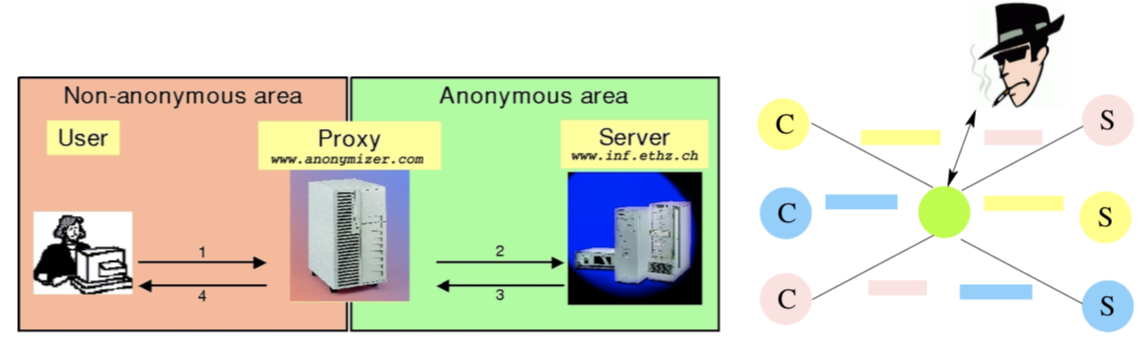
\includegraphics[scale=0.63]{proxy}
\end{figure}
\begin{multicols}{2}
	\noindent
	\textit{\textbf{Catene di proxy in cascata}}: ogni proxy conosce solo il \textit{next hop}. È ancora possibile effettuare \textit{traffic analysis}.
\columnbreak
	\begin{figure}[H]
		\centering
		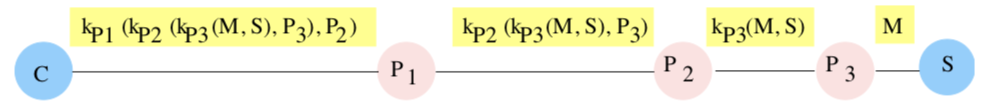
\includegraphics[scale=0.55]{proxycasc}
	\end{figure}
\end{multicols}
\begin{multicols}{2}
\noindent
\textit{\textbf{Mix Networks}}: è un meccanismo per la creazione di un \textit{canale anonimo}. È progettato per lavorare in un ambiente con un hacker attivo. Originariamente era stato proposto per sistemi di email anonime.\\\\
Un \textit{\textbf{Mix}} è un server che processa dei messaggi per $B$.\\
\begin{itemize}
	\item l'input del mix è la parte di sinistra;
	\item il Mix genera in output la parte di destra
	\item $R_i$ sono blocchi di stringhe di bit randomici.
\end{itemize}
\noindent
Questa è una variante di un \textit{single-proxy}. Il \textit{Mix} esegue anche altre operazioni per sconfiggere l'analisi del traffico.
\columnbreak
\begin{figure}[H]
	\centering
	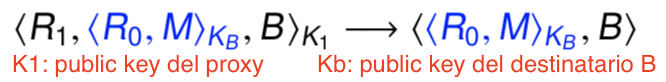
\includegraphics[scale=0.55]{mix}
\end{figure}
\begin{figure}[H]
	\centering
	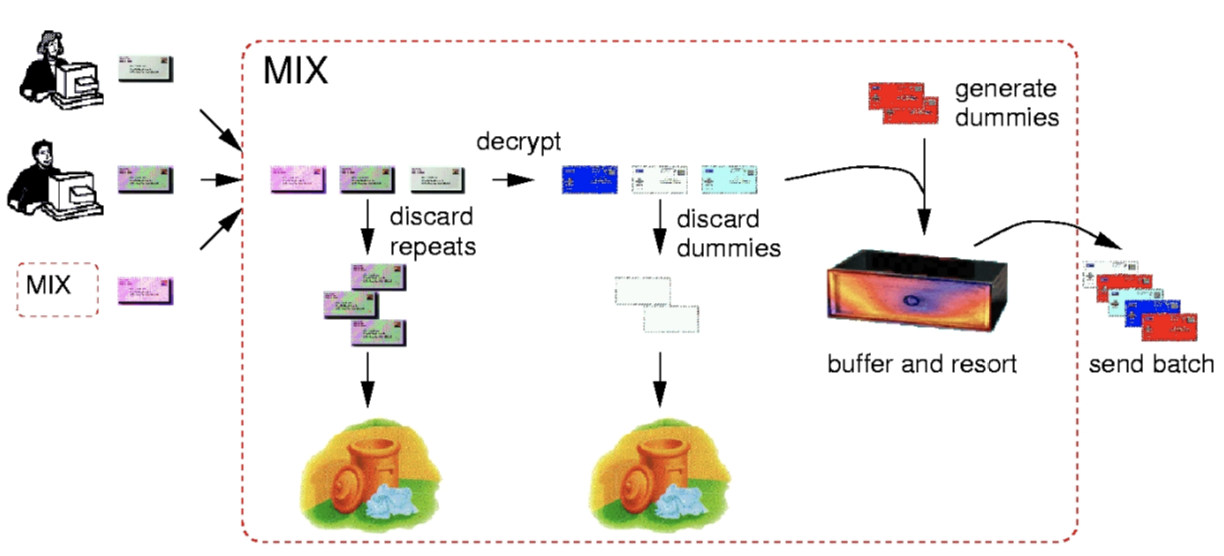
\includegraphics[scale=0.45]{mix2}
\end{figure}
\end{multicols}
\noindent
I \textit{Mix} lavorano con oggetti di dimensione uniforme (messaggi divisi in blocchi di dimensione fissa).\\
Ogni \textbf{Mix} riceve in input tanti messaggi da origini diverse (è meglio quando ci sono tante sorgenti), scarta i pacchetti ripetuti (per evitare i \textit{replay attack}), li decripta, scarta i pacchetti fittizzi, ne genera di nuovi (perché magari ci sono pochi utenti ed è necessario prevenire che i messaggi vengano tracciati), ne scambia l'ordine e li manda al \textit{next hop}.\\
Un \textit{single-mix} ha le stesse debolezze di un \textit{single-proxy}. È più sicuro averne tanti (in domini amministrativi diversi).\\
Se uno o più \textit{Mix} sono sotto il controllo di un hacker, è sufficiente che ne funzioni correttamente almeno uno.\\\\
Con questo funzionamento possiamo affermare che le \textbf{\textit{mix networks} garantiscono anonimità}. Non c'è correlazione tra input e output del \textit{mix}. Il \textbf{mittente resta anonimo} anche al destinatario.\\
\textit{\textbf{Svantaggi}}: nelle reti molto trafficate ci possono essere ritardi; è sufficiente ridurre o eliminare i pacchetti \textit{dummy}.
\begin{multicols}{2}
\begin{figure}[H]
	\centering
	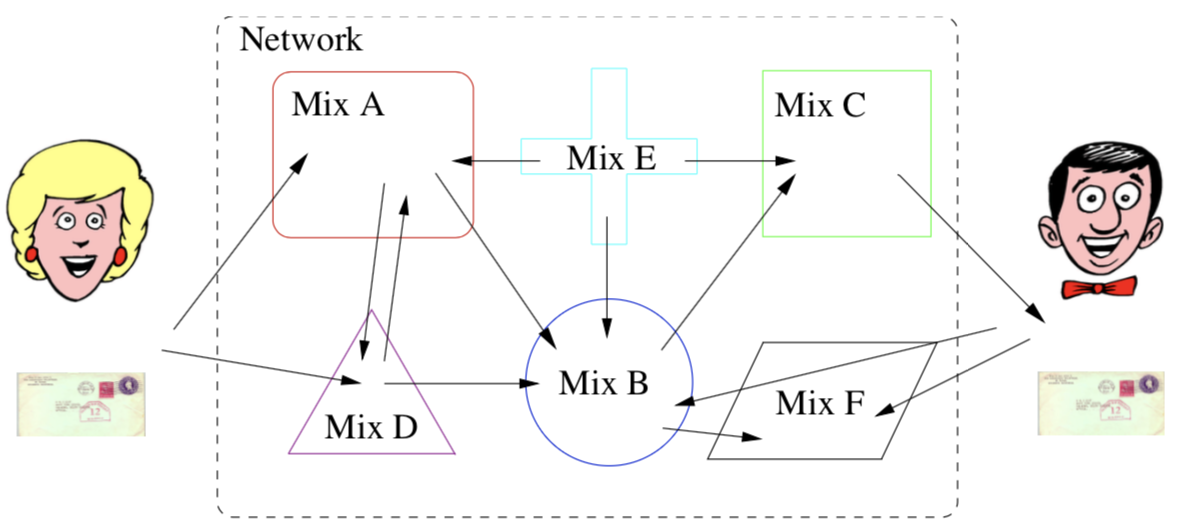
\includegraphics[scale=0.35]{dummy}
	\caption*{Con i \textit{dummy message} è difficile tracciare la conversazione.}
\end{figure}
\columnbreak
\setlength{\columnseprule}{0.4pt}
\begin{figure}[H]
	\centering
	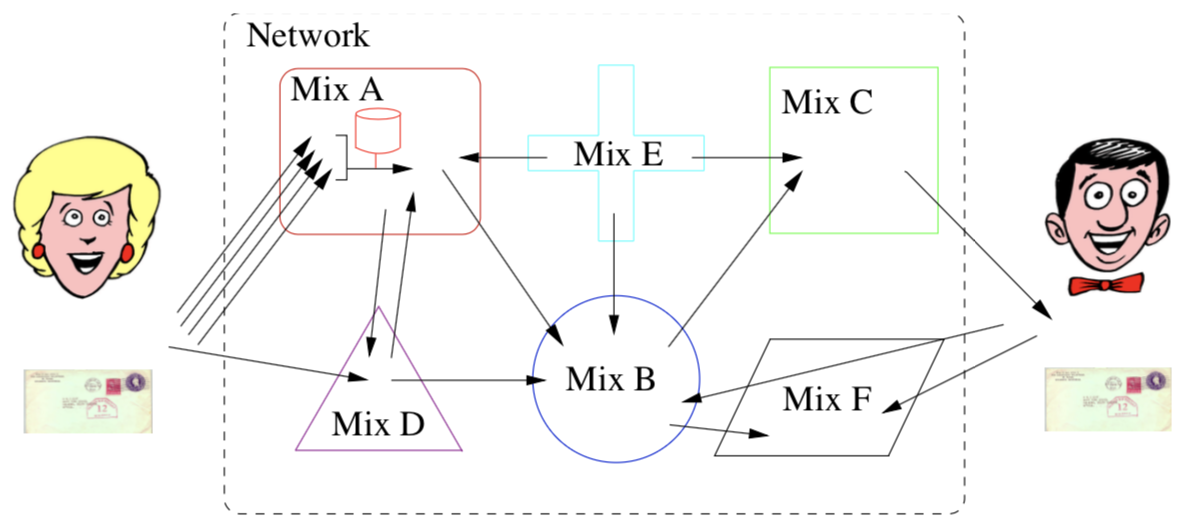
\includegraphics[scale=0.35]{replay}
	\caption*{Il \textit{replay filter} previene i \textit{replay attack}.}
\end{figure}
\end{multicols}

\noindent
Per \textbf{rispondere} ad un \textit{mittente anonimo}, esso deve includere $ \langle \langle R_1, \langle R_2, \dots \langle R_n, A_x \rangle_{K_n} \dots \rangle_{K_2} \rangle_{K_1}, K_x \rangle $ nel messaggio.\\
Il destinatario non potrà risalire all'IP di $A$ poiché resterà sempre criptato da stringhe randomiche $K_n$ scelte da $A$.\\
Il risultato finale ritornato ad $A$ sarà: ~$ \langle A_x, \langle \langle \langle \langle R_0, M \rangle_{K_x} \rangle_{R_1} \rangle_{R_2} \dots \rangle_{R_n} \rangle \ $.


\section*{Anonymity Network}
\addcontentsline{toc}{section}{Anonymity Network}
\begin{multicols}{2}
	\noindent
	\textbf{\textit{Internet}} è stato progettato come una \textbf{rete pubblica} e le informazioni di routing sono pubbliche (un ascoltatore passivo può sapere se due utenti stanno comunicando). La cifratura non nasconde le identità nei \textit{packet-headers}.\\\\
	L'\textit{\textbf{Anonimità}} è fondamentale nei sistemi utlizzati per certi scopi come: votazioni online, comunicazioni segrete, sistemi governativi o militari $\dots$\\
	Permette di renderdere un utente impossibile da identificare in mezzo ad altri utenti.
\columnbreak
	\begin{figure}[H]
		\centering
		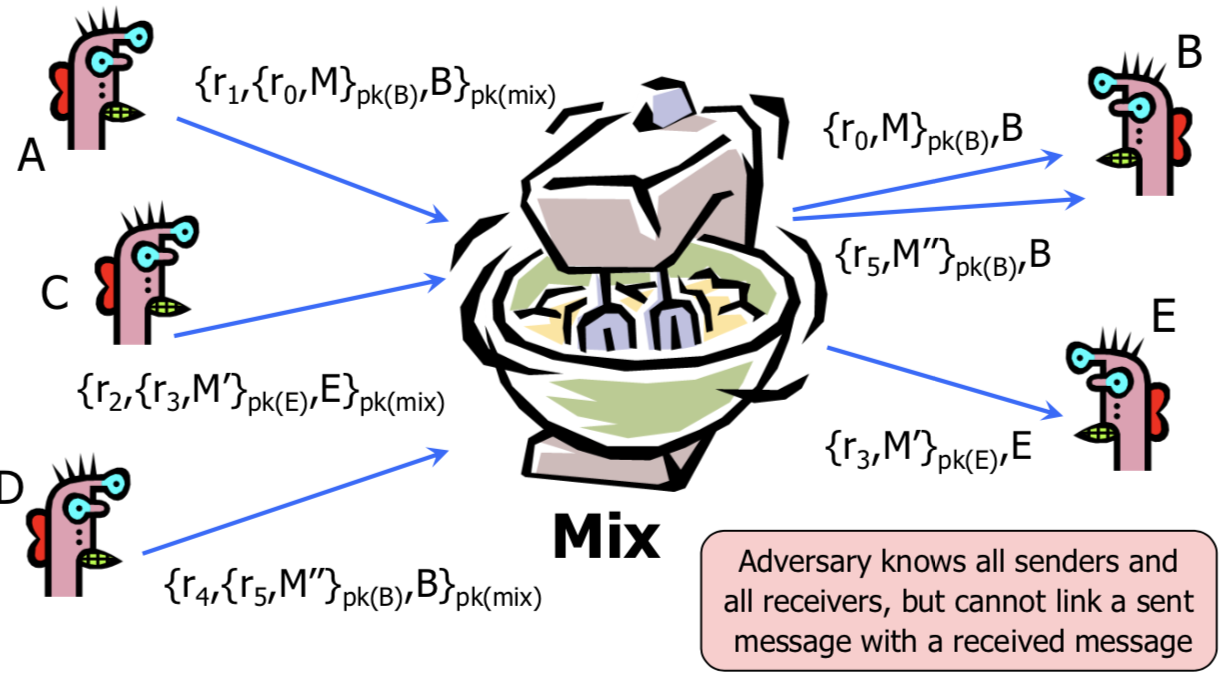
\includegraphics[scale=0.45]{mixan}
	\end{figure}
\end{multicols}
\noindent
Le \textit{Mix Networks} hanno una latenza eccessiva dovuta alla cifratura e decifratura a chiave pubblica (computazionalmente costosa). Questo ritardo è accettabile in un servizio di mail anonime ma non in \textit{web browser} anonimo.
\begin{multicols}{2}
	\noindent
	Un'idea può essere il \textbf{randomized routing} (utilizzato anche dall'\textit{Onion Routing}) che nasconde la sorgente di un messaggio attraverso un routing randomico. In questo modo i router non sanno se la sorgente apparente del messaggio è davvero il mittente oppure un altro router.
\columnbreak
	\begin{figure}[H]
		\centering
		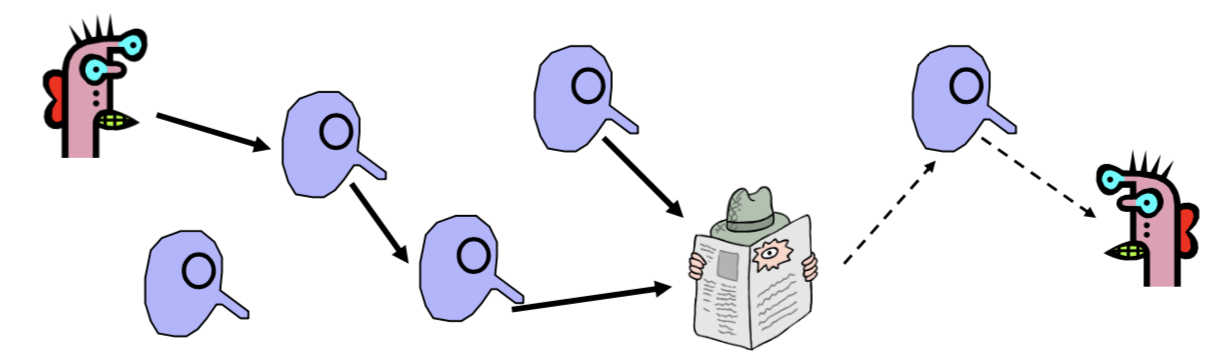
\includegraphics[scale=0.37]{randrout}
	\end{figure}
\end{multicols}
\begin{multicols}{2}
	\noindent
	\textit{\textbf{Onion Routing}}\\
	Il mittente scegli una sequenza randomica di router (alcuni possono essere sotto il controllo dell'hacker). Sceglie anche la lunghezza del percorso.\\
	Le informazioni di routing sono criptate con la \textit{public-key} del router che conosce solamente l'identità del successivo.
	\begin{figure}[H]
		\centering
		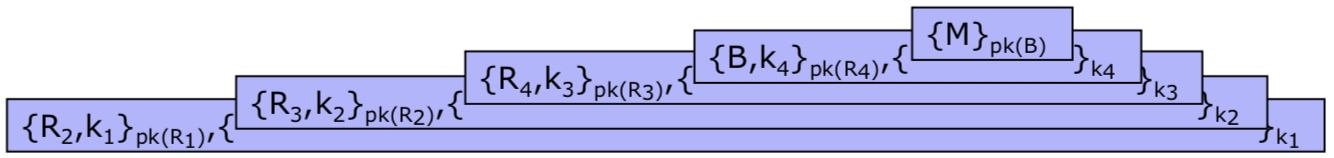
\includegraphics[scale=0.4]{onioninfo}
	\end{figure}
\columnbreak
	\begin{figure}[H]
		\centering
		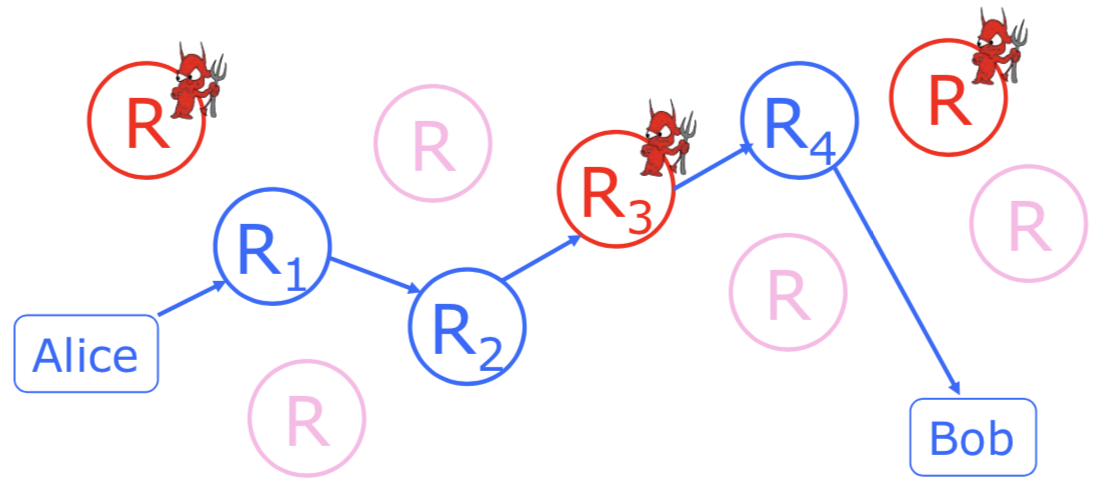
\includegraphics[scale=0.25]{onion}
	\end{figure}
	\begin{figure}[H]
		\centering
		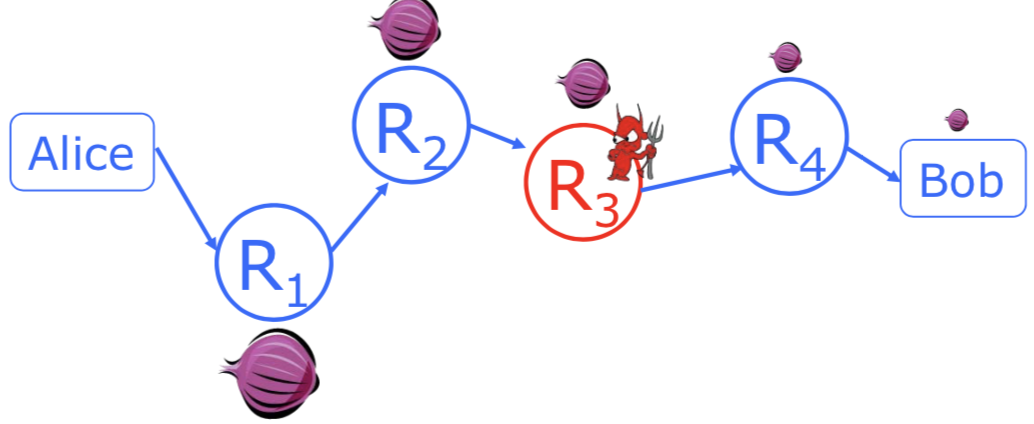
\includegraphics[scale=0.25]{onion2}
	\end{figure}
\end{multicols}


\subsubsection*{Tor}
\textit{\textbf{Tor}} è una \textit{onion routing network} di seconda generazione. Progettato per \textit{web browsing} anonimo a bassa latenza.
\begin{multicols}{2}
\begin{itemize}
	\item Il \textit{client-proxy} stabilisce \textit{session-key} simmetrica ed un circuito con gli \textit{Onion Router $\sharp1~\sharp2~\sharp3$} (tunnel).
	\item le applicazioni client si connettono e comunicano sul circuito \textit{Tor} stabilito.
	\item i datagrammi vengono decriptati e re-criptati ad ogni collegamento.
\end{itemize}
\columnbreak
\begin{figure}[H]
	\centering
	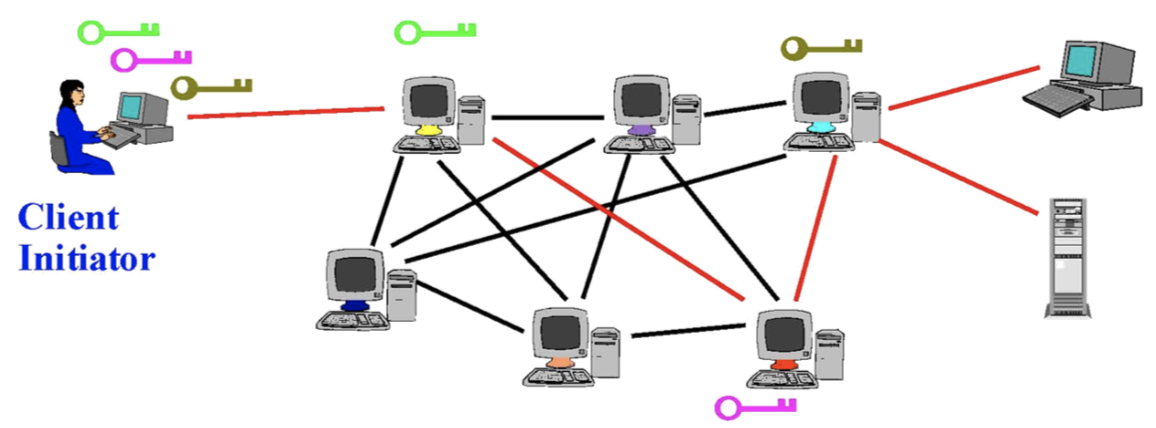
\includegraphics[scale=0.45]{tor}
\end{figure}
\end{multicols}
\noindent
\textit{\textbf{Problemi di gestione}}: \begin{itemize}
	\item molte applicazioni possono avviare troppe $TCP$ stream su un unico circuito;
	\item i router di \textit{Tor} non hanno bisogno di \textit{root-privileges}, incoraggiando le persone a settare i propri router (più partecipanti, più anonimità);
	\item \textit{directory server}: per tenere traccia degli onion router attivi, le loro locazioni e chiavi pubbliche, controllare i nuovi router che accedono alla rete (per evitare \textit{Sybil attack} in cui un attaccante crea tanti router), inviare la chiave del server con un codice \textit{Tor}.
\end{itemize}
\noindent
\textit{\textbf{Hidden Server}}: l'obiettivo è mettere online un server accessibile a tutti, ma che nessuno sappia dove si trova. Deve resistere alle censure, ai \textit{DoS attack} e non deve essere trovato fisicamente.
\begin{multicols}{2}
	\begin{figure}[H]
		\centering
		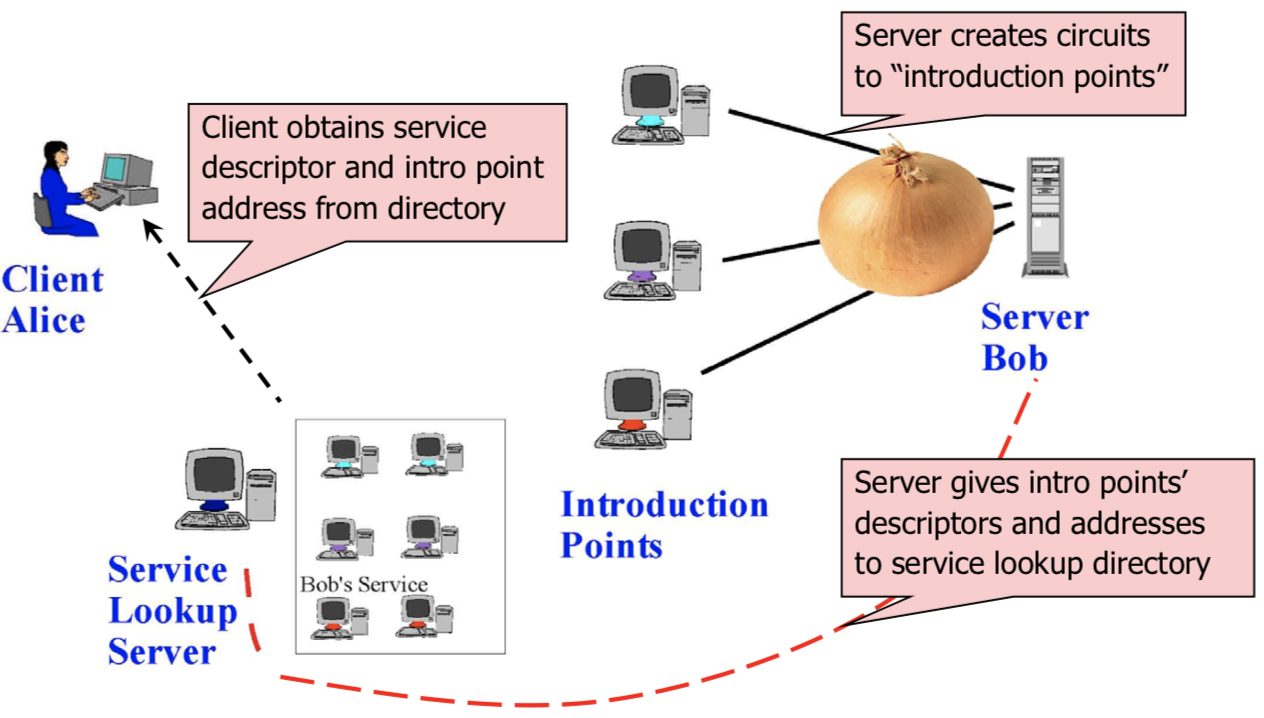
\includegraphics[scale=0.39]{hserver1}
	\end{figure}
\columnbreak
\setlength{\columnseprule}{0.4pt}
	\begin{figure}[H]
		\centering
		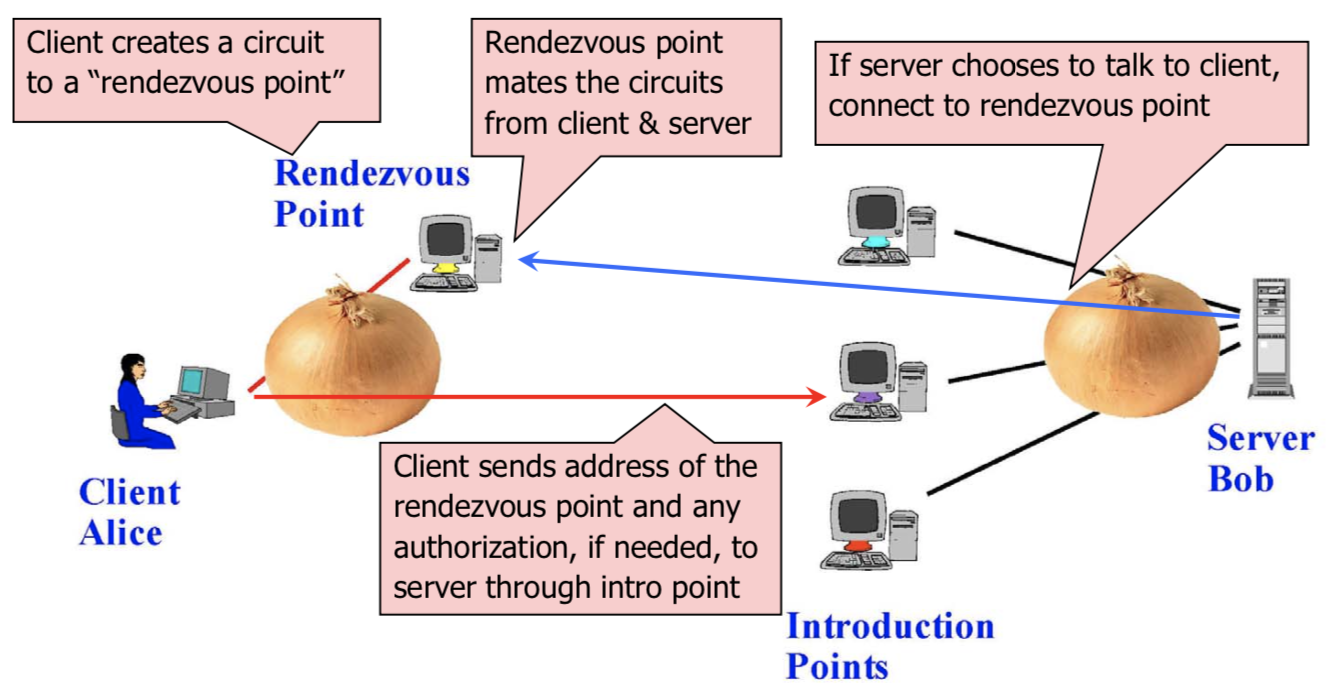
\includegraphics[scale=0.38]{hserver2}
	\end{figure}
\end{multicols}



\chapter*{Algoritmi e Meccanismi di Crittografia}
\addcontentsline{toc}{chapter}{Algoritmi e Meccanismi di Crittografia}
Un canale di comunicazione non affidabile può diventare sicuro applicando le 3 proprietà tramite la \textit{\textbf{Crittografia}}:
\begin{itemize}
	\item \textit{Confidentiality}: le informazioni trasmesse devono restare segrete;
	\item \textit{Integrity}: le informazioni non devono essere corrotte, alterate o eliminate;
	\item \textit{Authentication}: gli utenti devono sapere chi si trova dall'altro lato.
\end{itemize}
\noindent
Per criptare un messaggio si possono utilizzare algoritmi diversi:
\begin{multicols}{2}
\begin{itemize}
	\item \textbf{algoritmi simmetrici}: utilizzano la stessa chiave, oppure è semplice derivare una dall'altra;
\end{itemize}
\columnbreak
\begin{itemize}
	\item \textbf{algoritmi asimmetrici} o \textbf{chiave pubblica}: chiavi diverse, non derivabili tra loro; la pubblicazione della \textit{public key} non compromette la \textit{private key}.
\end{itemize}
\end{multicols}
\begin{multicols}{2}
	\begin{figure}[H]
		\centering
		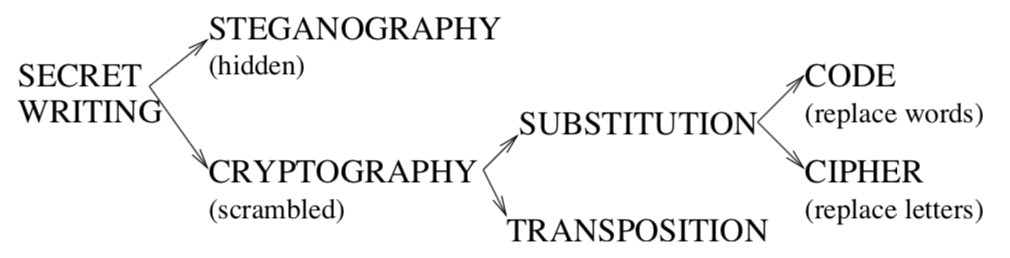
\includegraphics[scale=0.45]{hide}
	\end{figure}
\columnbreak
\begin{figure}[H]
	\centering
	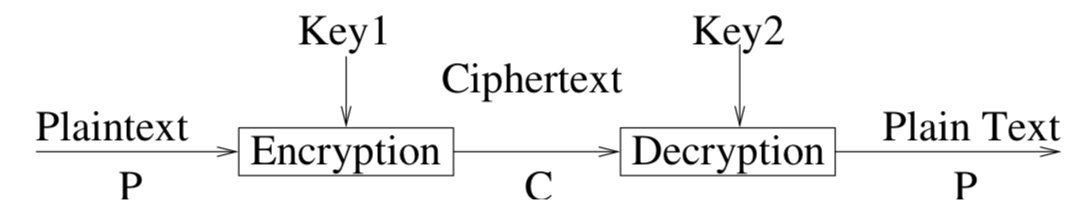
\includegraphics[scale=0.45]{keys}
\end{figure}
\end{multicols}

\noindent
Ci sono diverse classificazioni di sicurezza:
\begin{itemize}
	\item \textit{sicurezza incondizionale}: sistema sicuro anche se l'avversario ha un'infinita potenza di calcolo poiché il testo cifrato non ha abbastanza informazioni per risalire all'originale; la sicurezza si misura con la \textit{information theory}.
	\item \textit{sicurezza condizionale}: il sistema può essere attaccato ma sarebbe richiesta una potenza di calcolo irreale; la sicurezza è misurata usando la \textit{complexity theory}.
\end{itemize}

\noindent
\textit{\textbf{Cryptoanalysis}}: scienza che si occupa di recuperare un testo in chiaro partendo dal testo cifrato, senza chiave:
\begin{itemize}
	\item \textit{brute force attacks}: è sempre possibile, provando ogni chiave. È molto costoso sulla dimensione della chiave.
	\item \textit{cryptoanalitic attacks}: l'attaccante inizialmente conosce qualcosa (public key, plain texts $\dots$); un oracolo (informazioni che ottiene durante un attacco).
\end{itemize}


\section*{Simmetric Key Encryption}
\addcontentsline{toc}{section}{Simmetric Key Encryption}
Uno schema crittografico è a chiave simmetrica se per ogni coppia di chiavi $(e, d)$, esse sono uguali oppure è facile derivare una dall'altra. Conosciuti anche come: \textit{single-key}, \textit{one-key}, \textit{shared-key}, \textit{conventional encryption}.\\
Si può anche utilizzare il \textit{cifrario di Cesare}, oppure sostituire le lettere con la posizione nell'alfabeto.

\begin{multicols}{2}
\noindent
\textit{\textbf{Composite Ciphers}}: cifrare basandosi solo su sostituzioni o trasposizioni non è sicuro. È meglio una sostituzione seguita da una trasposizione. Difficile da fare a mano: invenzione delle macchine di cifratura (\textit{confusion and diffusion}).
\\
La fase di \textit{diffusion} nasconde la struttura del testo nel messaggio cifrato, la fase di \textit{confusion} rende molto complessa la relazione tra testo cifrato e chiave.\\
Un esempio pratico è la \textbf{Feisel Cipher Structure}.\\
Così come l'algoritmo \textbf{DES} (\textit{Data Encryption Standard}).
\columnbreak
\begin{figure}[H]
	\centering
	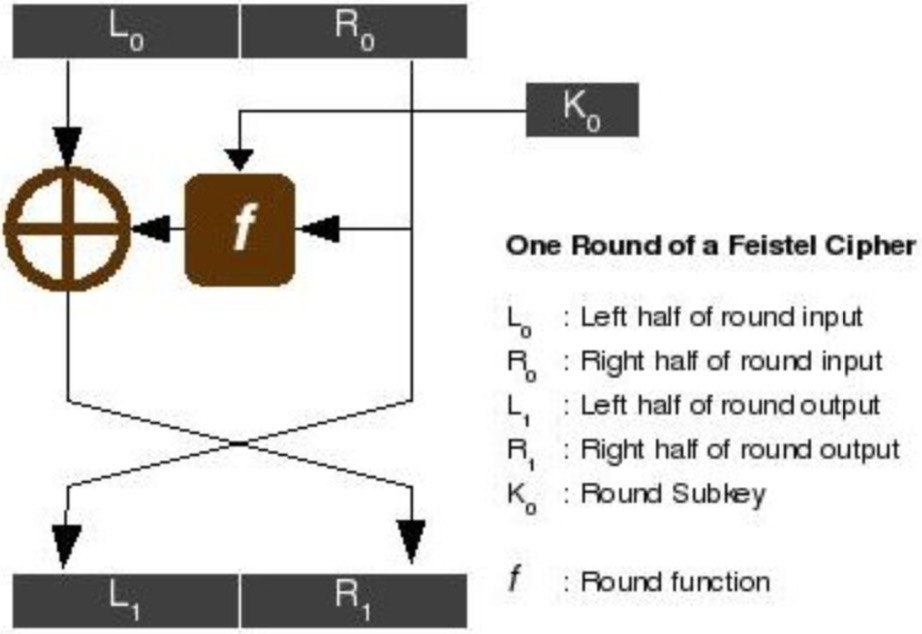
\includegraphics[scale=0.45]{feistel}
\end{figure}
\end{multicols}

\begin{multicols}{2}
\noindent
L'algoritmo \textbf{DES} si è rivelato essere poco sicuro perché la chiave usa solamente 56 bit per la cifratura dei blocchi di 64 bit. Raddoppiando il numero di chiavi (\textbf{Double DES}) non si ottiene un algoritmo con chiavi di 112 bit.\\ Resta esposto all'attacco \textit{Meet-in-the-Middle}.
\columnbreak
\begin{figure}[H]
	\centering
	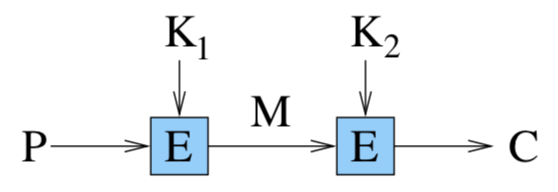
\includegraphics[scale=0.6]{doubleDES}
\end{figure}
\end{multicols}

\begin{multicols}{2}
	\noindent
	Triplicando le fasi crittografiche (\textbf{Triple DES}), usando le chiavi $K1$ e $K2$, si ottiene un algoritmo più sicuro poiché richiede un \textit{brute-force attack} di complessità 112 bit.\\
	Attualmente non esistono attacchi pratici all'algoritmo ed è compatibile con lo standard \textit{DES} ($K1 = K2$).
	\columnbreak
	\begin{figure}[H]
		\centering
		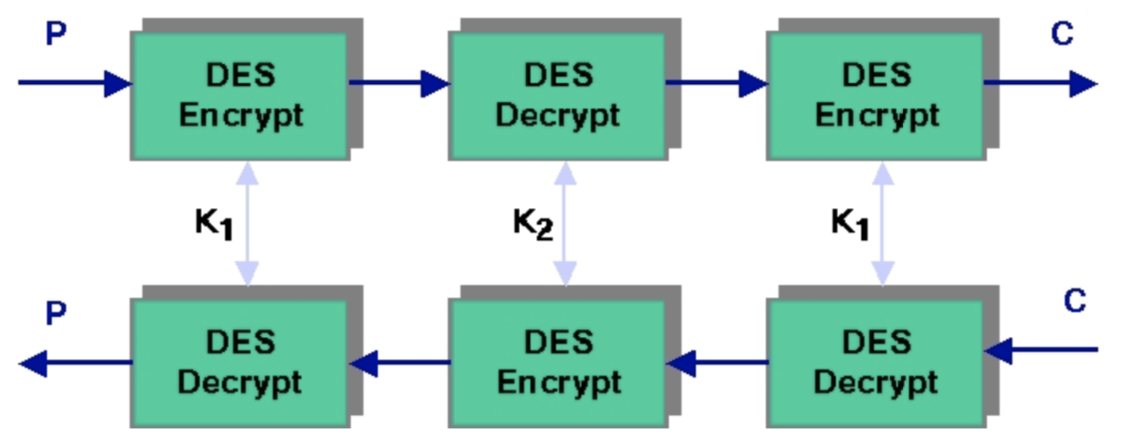
\includegraphics[scale=0.3]{tripleDES}
	\end{figure}
\end{multicols}
\noindent
Come successore di \textit{DES è stato proposto \textbf{AES}} (\textit{Advanced Encryption Standard}) che permette di criptare blocchi di 128, 192, 256 bit (non solo 64). Non usa la struttura di \textit{Feistal} ma processa l'intero blocco in parallelo.\\
Quando un messaggio supera la dimensione del blocco, dividerlo non è la soluzione migliore perché si possono perdere informazioni (stessi blocchi cifrati mappati sugli stessi blocchi in chiaro) e limitare l'integrità (la fase di decriptazione non indica se un blocco è stato cambiato, eliminato o duplicato).\\
È meglio fare lo XOR tra un blocco in chiaro e il precedecessore cifrato, così blocchi identici sono mappati in blocchi diversi cifrati. Se ci sono problemi al blocco $C_j$ ma non al blocco $C_{j+1}$, il blocco $C_{j+2}$ viene correttamente decriptato.


\subsection*{Placement of Encryption}
\addcontentsline{toc}{subsection}{Placement of Encryption}
\begin{multicols}{2}
	\noindent
\textit{\textbf{Link Encryption}}: la cifratura viene effettuata indipendentemente in ogni collegamento; il traffico deve essere decifrato e criptato ad ogni link (servono molti device, ma chiavi pari). Viene svolta al livello 1 o 2 dello stack OSI.
\\\\
\textit{\textbf{End-to-End Encryption}}: la cifratura avviene solo tra la sorgente e la destinazione; richiede chiavi condivise. Viene svolta ai livelli 3, 4, 6, 7 dello stack OSI (più sicuro).
\columnbreak
\begin{figure}[H]
	\centering
	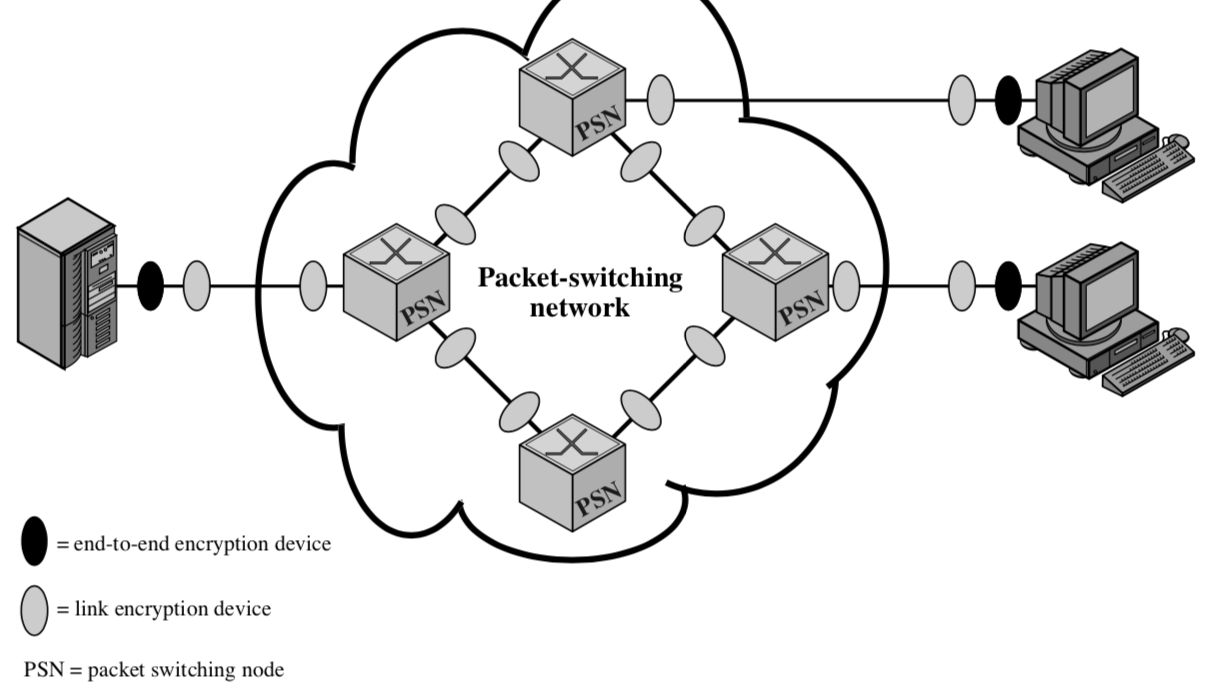
\includegraphics[scale=0.32]{eteenc}
\end{figure}
\end{multicols}
\noindent
Nella crittografia \textit{end-to-end}, gli headers vengono lasciati in chiaro per essere letti dalla rete e diretti alla destinazione. Idealmente, vorremmo poter criptare anche quelle informazioni per evitare che il monitoring della rete.


\subsection*{Key Distribution}
\addcontentsline{toc}{subsection}{Key Distribution}
Gli schemi simmetrici prevedono che entrambe le parti si scambino delle chiavi segrete comuni, in modo sicuro.
\begin{itemize}
	\item $A$ può selezionare la chiave e spedirla fisicamente a $B$;
	\item una terza parte può scegliere la chiave e spedirla ad $A$ e $B$;
	\item se $A$ e $B$ hanno comunicato in precedenza, possono utilizzare la chiave precedente per criptarne una nuova;
	\item se $A$ e $B$ hanno una comunicazione sicura con una terza parte $C$, allora $C$ può trasmettere la chiave tra $A$ e $B$.
	\newline
\end{itemize}

\begin{multicols}{2}
\noindent
Solitamente viene utilizzata una gerarchia di chiavi:
\begin{itemize}
	\item \textbf{Session key}: usata per la cifratura dei dati tra due utenti per una sessione e poi viene scartata;
	\item \textbf{Master key}: usata per criptare le \textit{session key}; condivisa tra gli utenti e il \textit{key distribution center}.
\end{itemize}
\columnbreak
\begin{figure}[H]
	\centering
	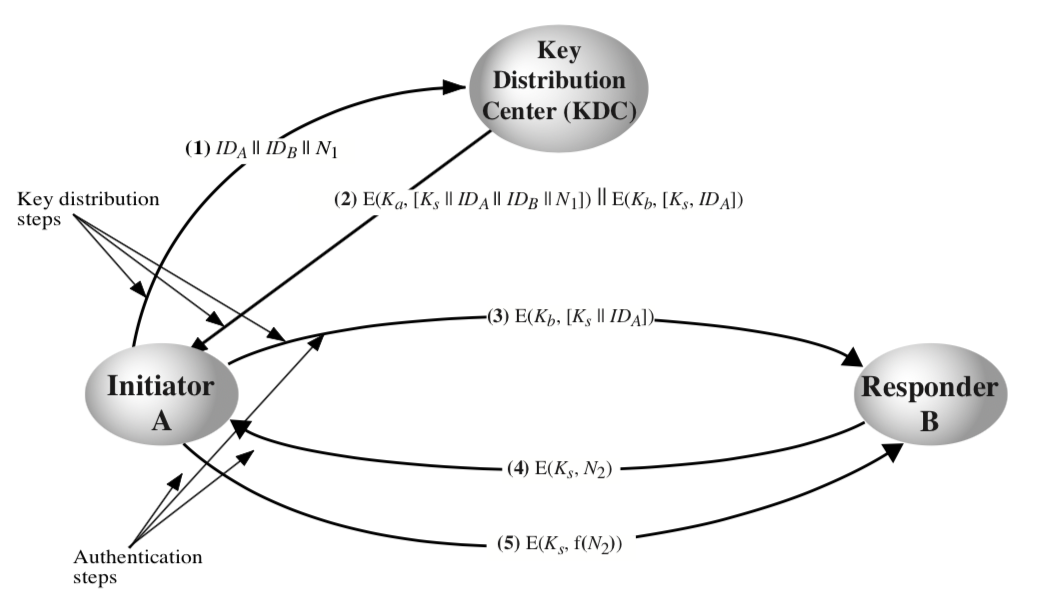
\includegraphics[scale=0.4]{keydist}
\end{figure}
\end{multicols}
\noindent
Le chiavi di sessione distribuite dal \textit{KDC} hanno un tempo di vita limitato per garantire maggiore sicurezza. Inoltre fa uso di un sistema di distribuzione automatico tra utenti (decentralizzato). Deve controllare l'utilizzo delle chiavi.













\chapter*{Algoritmi di Crittografia a Chiave Pubblica}
\addcontentsline{toc}{chapter}{Algoritmi di Crittografia a Chiave Pubblica}
La \textit{crittografia a chiave pubblica} nasce nel 1975 per risolvere due problemi: la distribuzione delle chiavi e la firma.\\
Considerando la coppia $(E_e, D_d)$, anche se $E_e$ è noto, è impossibile risalire da $c=E_e(m)$ a $m$; serve $D_d$. Per questo motivo si può affermare che la \textit{public key} può essere un'informazione pubblica (a differenza della \textit{private key}).\\\\
\textbf{Cifratura} di un messaggio $M$: $C = E(PU_{b}, M)$\\
\textbf{Decifratura} di un messaggio $C$: $M = D(PR_{b}, C) = D(PR_{b}, E(PU_{b}, M))$
\begin{multicols}{2}
	\begin{figure}[H]
		\centering
		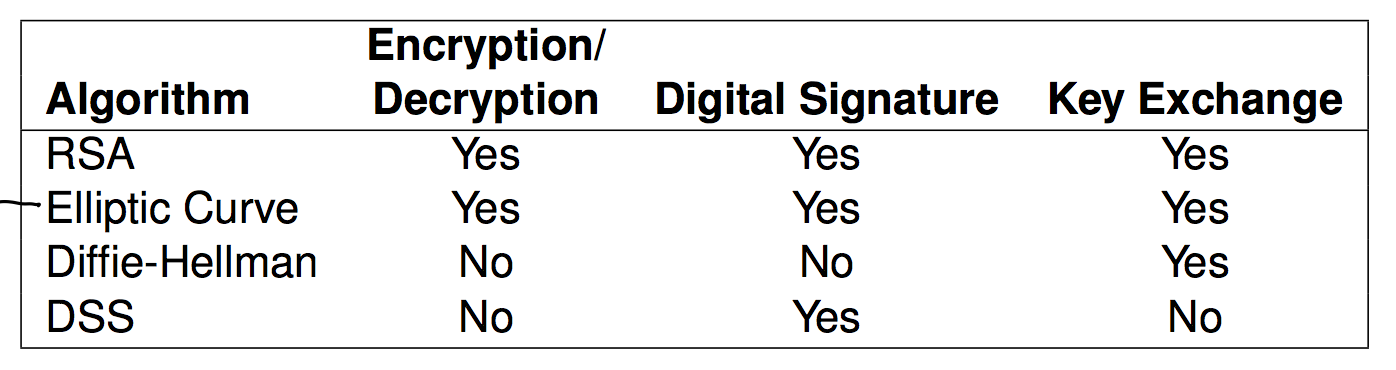
\includegraphics[scale=0.32]{confrontoalgoritmichiavepubblica}
	\end{figure}
	\columnbreak
	\begin{figure}[H]
		\centering
		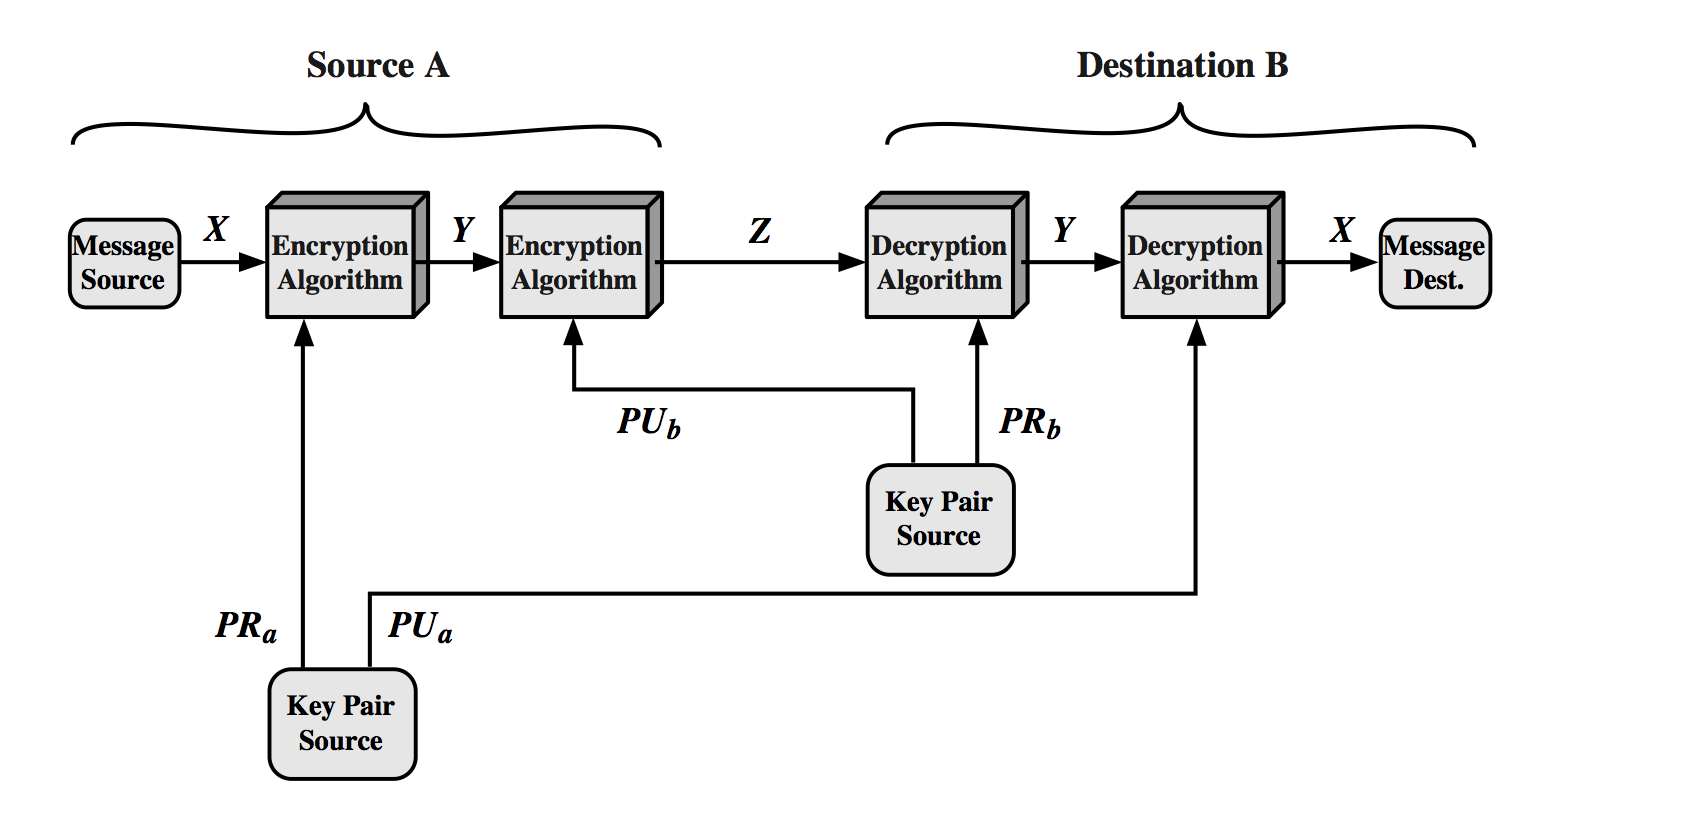
\includegraphics[scale=0.36]{secrecyauthenticationsicurezzareti}
	\end{figure}
\end{multicols}
\noindent
Un algoritmo di crittografia a chiave pubblica funziona come segue:
\begin{itemize}
	\item si utilizza lo stesso algoritmi per le fasi di \textit{encryption} e \textit{decryption} con una coppia di chiavi (una per fase);
	\item mittente e destinatario devono avere entrambi i tipi di chiave (non uno solo).
	\newline
\end{itemize}
\noindent
Un algoritmo di crittografia a chiave pubblica, per la sicurezza ha bisogno delle seguenti proprietà:
\begin{itemize}
	\item una delle due chiavi deve rimanere segreta;
	\item è praticamente impossibile decifrare un messaggio senza informazioni aggiuntive;
	\item conoscere l'algoritmo, una sola chiave e dei modelli del testo cifrato non è sufficiente per risalire all'altra chiave.
\end{itemize}

\noindent
Un destinatario $B$ genererà le chiavi $PU_b$ e $PR_b$, il mittente $A$ conoscerà $PU_b$ e $M$ per generare $C = E (PU_b, M)$; il destinatario $B$ potrà decriptare $C$ con $PR_b$. L'avversario, dati $PU_b$ e $C$, non riesce a ricostruire $M$.\\
Questo si ha perché l'algoritmo si basa su una \textbf{one-way function}: data $f: X \rightarrow Y$, $f$ è facile da calcolare per ogni $x\in X$, ma $f^{-1}$ è difficile da trovare.\\
Si basa inoltre sul concetto di \textbf{trapdoor function}: una funzione $f_{k}: X \longrightarrow Y$ che data una informazione extra $k$, è semplice trovare per $y \in Im(f)$, $x \in X$ dove $f_{k}(x) = y$

\subsubsection*{Public-key Cryptoanalysis}
\begin{itemize}
	\item \textit{Brute-force attacks}: la contromisura consiste nell'utilizzo di chiavi grandi; è però necessario un tradeoff per non aumentare troppo la complessità delle fasi di encryption/decryption.
	\item \textit{Computing private key from public key}: non ci sono prove che questo attacco sia irrealizzabile.
	\item \textit{Probable-message attack}: supponendo di avere un messaggio $M$ di pochi bit (es. 56bit) criptato con la $PU_a$, l'attaccante può calcolare tutti i possibili $Y_i = E(PU_a, X_i)$ per tutti i possibili messaggi $X_i, i = 1 \dots 2^{56}$! La soluzione consiste nell'aggiungere bit random a $M$.
\end{itemize}



\section*{Algoritmo RSA}
\addcontentsline{toc}{section}{Algoritmo RSA}
Algoritmo pubblicato nel 1976 e nominato nel 1978 dagli inventori Rivest, Shamir, Adleman.\\
La sua sicurezza è data dalla difficoltà di fattorizzare grandi numeri. Le chiavi sono funzioni di coppie di grandi numeri primi (oltre 100 cifre). È l'algoritmo a chiave pubblica più popolare, utilizzato in molte applicazioni (PGP, SSL $\dots$).\\
Risolve il problema della gestione delle chiavi ma ha alcuni \textbf{svantaggi}: lentezza, ha bisogno di chiavi grandi ed è vulnerabile ad alcuni attacchi (\textit{plaintext} e \textit{timing attacks}).
\subsection*{Number Theory}
\begin{itemize}
	\item \textit{Prime Factorization}: scrittura di un numero come prodotto di numeri primi.
	\item \textit{Relative Prime Numbers \& MCD}: due numeri sono relativamente primi se non hanno divisori comuni; tra due numeri si può trovare anche il \textit{massimo comune divisore}.
	\item \textit{Modular Arithmetics}: $\forall a, n. \exists q, r . (a = q * n + r)$ con $0 \leq r < n < a$, il resto $r = a~mod~n$.\\
	$a, b \in \mathbb{Z}$ sono \textit{congruenti modulo n} se $a~mod~n=b~mod~n$ e si scrive con $a=_n b$.
	\item \textit{Euler Totient Function}: facendo il modulo $n$ si ha un insieme completo di resti di cui si tengono solamente i numeri primi (\textit{reduced set of residues}), il cui numero di elementi è chiamato \textbf{Euler Totient Function} $\phi(n)$.
\end{itemize}

\begin{thm}[Fermat's little theorem]\label{thm:TeoremaFermat}
	Per $a$ e $n$ primi tra loro ed $n$ primo, ~~$a^{n-1} =_{n} 1 $
\end{thm}
\noindent
Considerato $a$ $mod$ $n$:\\
\textbf{Residui}: $0,\dots, n-1$ \\
\textbf{Set di residui ridotto}: \textit{residui che sono primi tra loro con n}\\
Il numero di elementi nel \textbf{set di residui ridotto} è chiamata \textbf{funzione di totient di Eulero}: $\phi(n)$\\
Proprietà:
\begin{itemize}
	\item $\phi(1)=1$
	\item $\phi(p) = p-1$ se $p$ è primo
	\item $\phi(p*q) = \phi(p)*\phi(q) = (p-1)*(q-1)$ se $p$ e $q$ sono primi e $p \neq q$
\end{itemize}
~\\
Il \cref{thm:TeoremaFermat} può essere riscritto come:
\begin{thm}[Teorema di Eulero]
	$a^{\phi(n)} =_{n} 1$ per tutti gli $a, n$ tali che $MCD(a,n) = 1$
\end{thm}


\subsection*{Funzionamento}
\textbf{Cifratura}: $C = M^{e}$ $mod$ $n$ \\
\textbf{Decifratura}: $M = C^{d}$ $mod$ $n = (M^{e})^{d}$ $mod$ $n = M^{ed}$ $mod$ $n$ \\
\textbf{Chiave pubblica}: $PU = {e,n}$\\
\textbf{Chiave privata}: $PR = {d,n}$\\
~\\
\textbf{Generazione chiavi:}
\begin{itemize}
	\item Generare due numeri primi $p$ e $q$ distinti e molto grandi;
	\item Computare $n = pq$ e $\phi = (p-1)(q-1)$
	\item Selezionare $e$ tc. $1 < e < \phi$ relativamente primo a $\phi$;
	\item Computare $d = e^{-1}$ $mod$ $\phi$;
	\item Chiave pubblica = $(e, n)$\\
	Chiave privata = $(d, n)$
\end{itemize}
\noindent
Un eventuale progresso futuro nella \textit{teoria dei numeri} potrebbe rendere \textbf{RSA} insicuro poiché si basa sulla difficoltà di effettuare certe computazioni in un tempo ragionevole.
\begin{multicols}{2}
\noindent
\textbf{Criptazione:}
\begin{itemize}
	\item Dividere il messaggio in blocchi $M_{1}, M_{2} \dots$ con $M_{i} < n$
	\item Computare $C_{i} = M_{i}^{e}$ $mod$ $n$
\end{itemize}
\columnbreak
\noindent
\textbf{Decriptazione:}
\begin{itemize}
	\item Computare $M_{i} = C_{i}^{d}$ $mod$ $n = (M^e)^d$ $mod$ $n = M^{ed}$ $mod$ $n$
	\newline
	\newline
\end{itemize}
\end{multicols}

\subsection*{Condivisione Segreta delle Chiavi con RSA}
Essendo la crittografia a chiave pubblica molto onerosa dal punto di vista computazionale, si ricorre alla crittografia simmetrica, in cui lo scambio iniziale delle chiavi avviene utilizzando la crittografia asimmetrica.
\begin{multicols}{2}
\noindent
\textbf{Criptazione (con chiave pubblica $(e, n)$):}
\begin{itemize}
	\item Scegliere randomicamente $k$
	\item $C = (k^{e}$ $mod$ $n,$ $E_{k}(m))$
\end{itemize}
\columnbreak
\noindent
\textbf{Decriptazione (con chiave privata $(d, n)$):}
\begin{itemize}
	\item Splittare il messaggio $C$ in $(c_{1}, c_{2})$
	\item $k = c_{1}^{d}$ $mod$ $n$ \\
	$m = D_{k}(c_{2})$
\end{itemize}
\end{multicols}
\noindent
\textbf{Problema}: se la private-key $(d, n)$ è compromessa, $k$ può essere recuperata da un intruso che registra la conversazione.

\section*{Algoritmo di Diffie-Hellman}
\addcontentsline{toc}{section}{Algoritmo di Diffie-Hellman}

\subsection*{Fondamenti matematici}
Una \textbf{radice primitiva} $s$ di un numero primo $p$ è un numero le cui potenze generano $1, \dots, p-1$. Così $s$ $mod$ $p, \dots$ $s^{p-1}$ $mod$ $p, \dots$ sono permutazioni distinte da $1$ a $p-1$. Quindi \[ \forall b \in \mathbb{Z}.\ \exists i \in \{0, \dots, p-1\}.\ b = s^{i}\ mod\ p \]
Dato $b \in \mathbb{Z}$, l'esponente $i$ è \textbf{il logaritmo discreto} di $b$ per la base $s$, $mod\ p$. Computare \textbf{logaritmi discreti} sembra essere computazionalmente impossibile.
\subsection*{Funzionamento}
L'obiettivo è lo scambio di una chiave condivisa tra due attori:
\begin{enumerate}
	\item Gli attori $A$ e $B$ si scambiano un \textit{numero primo $q$ e una radice primitiva $\alpha$}, entrambi pubblicamente visibili;
	\item $A$ e $B$ generano numeri casuali $X_{A}$ e $X_{B}$, rispettivamente minori di $q$;
	\item $A$ computa $Y_{A} = \alpha^{X_{A}}\ mod\ q$, $B$ computa $Y_{B} = \alpha^{X_{B}}\ mod\ q$;
	\item $A$ e $B$ si scambiano i risultati;
	\item $A$ computa $K_{A} = Y^{X_{A}}_{B}\ mod\ q$, $B$ computa $K_{B} = Y^{X_{B}}_{A}\ mod\ q$. Le \textbf{chiavi} sono \textbf{uguali}, infatti: \[ K_{A} = Y^{X_{A}}_{B}\ mod\ q = (\alpha^{X_{B}})^{X_{A}}\ mod\ q = (\alpha^{X_{A}})^{X_{B}}\ mod\ q \]
\end{enumerate}
\noindent
\textbf{Punti di forza:}
\begin{itemize}
	\item La chiave condivisa è creata dal nulla;
	\item La chiave condivisa ottenuta è almeno potente quanto la \textit{half-key};
	\item La chiave condivisa non è mai trasmessa, se non in forma criptata (si scambiano le \textit{half-key});
	\item \textbf{Perfect Forward Secrecy (PFS)}: una chiave di sessione derivata da un insieme di chiavi private e pubbliche non sarà mai compromessa se una di esse viene violata. Verranno violati solamente i dati criptati con le chiavi compromesse.
\end{itemize}
\noindent
Se qualcuno dovesse scoprire le chiavi private dopo aver registrato l'intera conversazione, non sarebbe comunque in grado di decriptare nulla (tranne i dati esplicitamente criptati con quella chiave privata).\\
Questo algoritmo gode comunque della proprietà di \textbf{scalabilità} poiché può essere esteso a 3 o più utenti.
\newpage
\noindent
\textbf{Debolezze:}
vulnerabile a \textbf{MitM attack} nella variante non autenticata.
\begin{itemize}
	\item $A$ trasmette $Y_{A}$ a $B$
	\item $Z$ (l'attaccante) intercetta $Y_{A}$ e trasmette $Y_{Z}$ a $B$. Calcola anche $K_{1} = (Y_{A})^{X_{Z}}\ mod\ q$
	\item $B$ riceve $Y_{Z}$ e calcola $K_{2} = (Y_{Z})^{X_{B}}\ mod\ q$
	\item $B$ trasmette $Y_{B}$ ad $A$
	\item $Z$ intercetta $Y_{B}$ e trasmette $Y_{Z}$ ad $A$. Calcola anche $K_{2} = (Y_{B})^{X_{Z}}\ mod\ q$
	\item $A$ riceve $Y_{Z}$ e calcola $K_{1} = (Y_{Z})^{X_{A}}\ mod\ q$
\end{itemize}
\noindent
In questo caso $A$ pensa di condividere una secret-key ma sta condividendo $K_1$ con $Z$, mentre $B$ condivide $K_2$ con $Z$.\\
Ciò è dovuto alla \textbf{mancanza di autenticazione} tra $A$ e $B$ (non c'è nessuna violazione essendo su canale pubblico).

\begin{figure}[H]
	\centering
	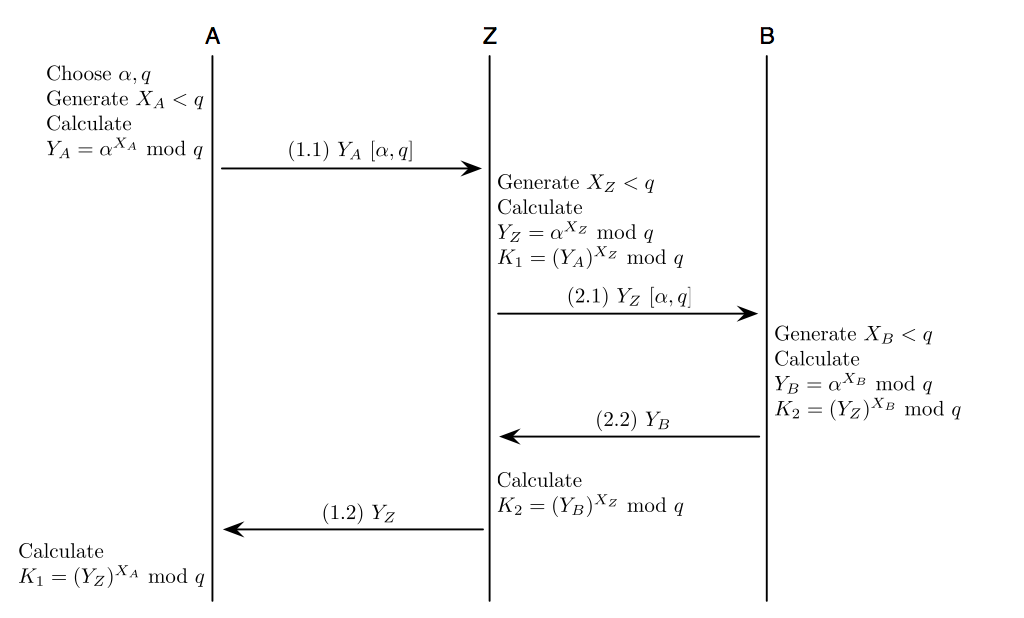
\includegraphics[scale=0.6]{diffiehellmanmitm}
\end{figure}


\section*{ElGamal (Variante di Diffie-Hellman)}
\addcontentsline{toc}{section}{ElGamal (Variante di Diffie-Hellman)}
\subsection*{Funzionamento}
Simile a \textbf{Diffie-Hellman}: al passo 2 viene già inviato il messaggio criptato
	\begin{enumerate}
		\item $B$ calcola $Y_B=\alpha^{X_B}$ $mod$ $q$ e poi $B \longrightarrow A:\ Y_{B}$
		\item $A$ calcola $Y_A=\alpha^{X_A}$ e anche $K=Y_B^{X_A}$ $mod$ $q$; infine $A \longrightarrow B:\ (E(M,K), Y_{A})$
		\item $B$ computa $K = Y_{A}^{X_{B}}\ mod\ q$ e usa $K$ per decriptare $E(M,K)$ 
	\end{enumerate}

\section*{Massey-Omura}
\addcontentsline{toc}{section}{Massey-Omura}
\subsection*{Funzionamento}
Criptazione senza chiavi condivise, si basa sul problema del logaritmo discreto, condividendo un numero primo $p$;
\begin{itemize}
	\item $u \in \{A,B\}$ sceglie $e_{u}, d_{u} \in \mathbb{Z}$ in modo privato, tale che: $ e_{u}d_{u}\ mod\ (p-1) = 1 $\\ Quindi $(p-1)$ divide $(e_{u}d_{u} -1)$. Ricordando che se $a/b \longmapsto a = q*b+r$, esiste un $k$ dove $e_{u}d_{u} = k(p-1)+1$. Dal teorema di Eulero, $\forall m \in \{1,\dots p-1\}$ \[ m^{e_{u}d_{u}}\ mod\ p = m^{k(p-1)}m\ mod\ p = m\ mod\ p = m \]
	\item Schema:
	\begin{enumerate}
		\item $A \longrightarrow B:\ m^{e_{A}}\ mod\ p$
		\item $B \longrightarrow A:\ m^{e_{A}e_{B}}\ mod\ p$
		\item $A \longrightarrow B:\ m^{e_{A}e_{B}d_{A}}\ mod\ p$ $(= m^{e_{B}})$
		\item $A \longrightarrow B:\ m^{e_{A}e_{B}d_{A}d_{B}}\ mod\ p$ $(= m)$
	\end{enumerate}
\end{itemize}
\noindent
Anche in questo caso $A$ NON è certa di scambiare messaggi con $B$: ancora possibile \textbf{MitM attack}.



\chapter*{Integrità dei Messaggi e Hash Crittografici}
\addcontentsline{toc}{chapter}{Integrità dei messaggi e hash crittografici}
\section*{Hash}
\addcontentsline{toc}{section}{Hash}
Per integrità del dato si intende la proprietà che esso non sia in qualche modo alterato da terze parti.\\
Si vuole creare un'impronta digitale del dato, cioé una \textbf{funzione di hashing $h(x)$}, che ha le seguenti proprietà:
\begin{enumerate}
	\item \textit{Compressione:} $h$ mappa un'input $x$ di lunghezza arbitraria, in un output $h(x)$ di lunghezza fissata $n$;
	\item Calcolabile in tempo polinomiale.
\end{enumerate}
$h(x)$ è inoltre \textbf{una funzione di hashing crittografica} se:
\begin{enumerate}
	\item è \textit{non invertibile} (detta anche proprietà di \textit{pre-image resistant})
	\item solitamente anche:
	\begin{itemize}
		\item \textit{2-nd preimage resistant}: impossibile trovare un secondo input che ha lo stesso output del primo, cioè dato $x$, è difficile trovare $x'\neq x.\  h(x)=h(x')$ 
		\item \textit{Collision resistance}: difficile trovare due input distinti $x, x'.\ h(x)=h(x')$ 
	\end{itemize}
\end{enumerate}
\noindent
Per costruire una \textit{funzione di hash crittografica} si può usare la tecnica della \textbf{block chain}: l'output dell'encoding di un blocco viene dato in input al seguente per essere utilizzato nell'encoding dello stesso (e così via per gli altri blocchi).


\section*{MAC}
\addcontentsline{toc}{section}{MAC}
L'obiettivo è sempre quello di mantenere l'\textbf{authentication integrity} per verificare che nessuno alteri la conversazione.\\
Il \textit{\textbf{Message Authentication Code (MAC)}} e la firma digitale sono le due tecniche principali per l'autenticazione.\\
Un algoritmo MAC è una famiglia di funzioni di hash $h_{k}$ parametrizzate da una chiave segreta $k$ condivisa. 
$h_{k}$ deve essere \textit{computazionalmente resistente}: date $0$ o più coppie MAC $(x_{i}, h_{k}(x_{i}))$ non è fattibile computare $(x, h_{k}(x))$ per ogni nuovo input $x \neq x_{i}$ (è impossibile calcolare l'hash se non si conosce la chiave segreta $k$).\\
Non c'è però il controllo sui \text{message replay} (la firma può essere scaduta), dunque non assicura \textit{freshness}.

\begin{figure}[H]
	\centering
	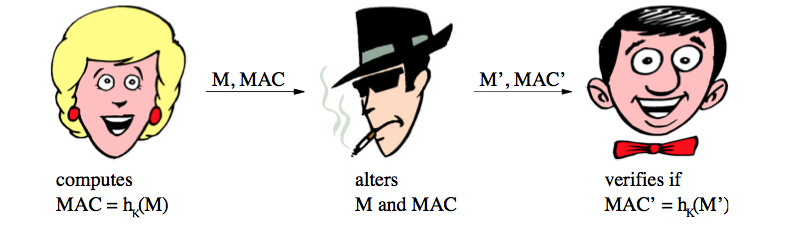
\includegraphics[scale=0.52]{macscheme.png}
\end{figure}

\subsection*{Costruire un algoritmo MAC}
\begin{multicols}{2}
\noindent
Una realizzazione si basa sulla \textit{cipher-block chaining}.\\
$c_1 = E_K (m_1 + 0)$\\
$c_i = E_K (c_{i-1} + m_i)$\\
$E$ è un blocco cifrato (es. \textit{DES}), $c_n$ è il \textit{MAC}.
\columnbreak
\begin{figure}[H]
	\centering
	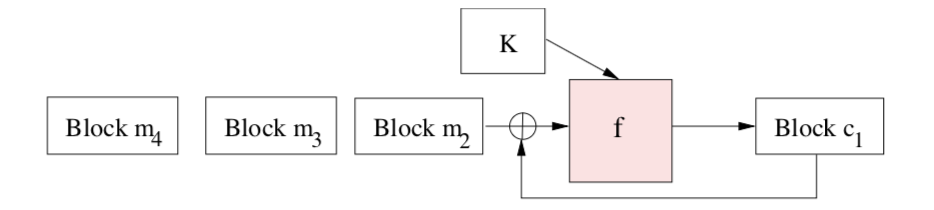
\includegraphics[scale=0.55]{maccostruction.png}
\end{figure}
\end{multicols}

\section*{Firma digitale}
\addcontentsline{toc}{section}{Firma digitale}
Problema della prova dell'origine dei dati: si può essere sicuri che il messaggio provenga da una persona specifica (\textbf{proprietà di non ripudio}) utilizzando una chiave condivisa?\\
La firma digitale è fondamentale per l'autenticazione e il \textit{non ripudio} dei messaggi.\\
Sono tuttavia possibili i \textit{replay attack} poiché le firme possono essere scadute.

\subsection*{Nomenclatura}
\begin{itemize}
	\item $M$ è l'insieme dei messaggi che possono essere firmati;
	\item $S$ è l'insieme delle firme, cioè stringhe di $n$ bit;
	\item $S_{A}: M \longrightarrow S$ è la trasformazione corrispondente alla firma per $A$, tenuta segreta da $A$;
	\item $V_{A}: M \times S \longrightarrow \{true,false\}$ è la funzione di verifica per $A$ ed è nota pubblicamente (prende un messaggio ed una firma: ritorna \textit{true} se c'è corrispondenza);
	\item $S_{A}$ e $V_{A}$ forniscono uno schema di \textbf{firma digitale per $A$}
\end{itemize}

\subsection*{Costruzione di uno schema di firma}
\begin{multicols}{2}
	\begin{itemize}
		\item \textit{Signing procedure}: $A$ crea una firma per $m\in \mathcal{M}$ creando $s=S_A(m)$ e trasmettendo la coppia $(m,  s)$.
		\item \textit{Verification procedure}: $B$ verifica la firma di $A$ su $(m, s)$ calcolando $u=V_A(m, s)$ e la accetta se ritorna \textit{true}.
		\item \textit{Secrecy requires}: è difficile per un'entità diversa da $A$ trovare, per ogni $m\in \mathcal{M}$ un $s\in \mathcal{S}$, tale che $V_A(m, s) = true$.
	\end{itemize}
\columnbreak
\begin{figure}[H]
	\centering
	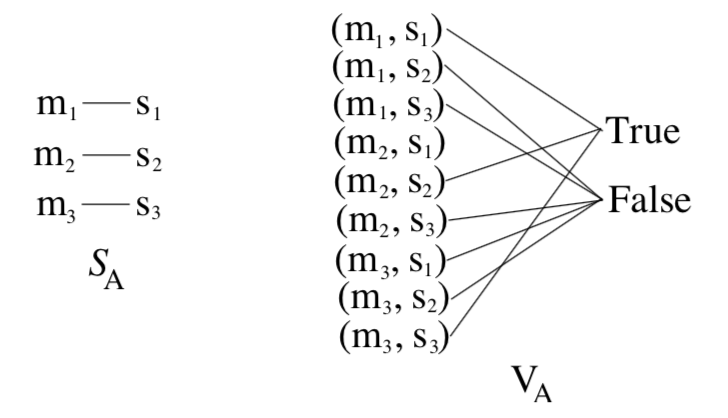
\includegraphics[scale=0.6]{signatureschema.png}
\end{figure}
\end{multicols}
\noindent
L'implementazione della firma digitale si può basare sui sistemi (reversibili) di crittografia a chiave pubblica.\\
Sia $E_e: \mathcal{M} \rightarrow \mathcal{C}$ una trasformazione a chiave pubblica e supponiamo che $\mathcal{M} = \mathcal{C}$. Se $D_d$ è la funzione di decriptazione corrispondente a $E_e$, allora entrambe sono permutazioni:
$$ D_d(E_e(m)) = E_e(D_d(m)) = M \text{~~~~per ogni~~} m\in \mathcal{M} $$
\noindent
Questo schema di crittografia a chiave pubblica è chiamato \textit{reversibile}.\\
La costruzione dello schema per la firma digitale avviene come segue:
\begin{itemize}
	\item siano $\mathcal{M}$ e $\mathcal{C}$ un messaggio e uno spazio di firma con $\mathcal{M} = \mathcal{C}$;
	\item sia $(e, d)$ una coppia di chiavi per lo schema di crittografia a chiave pubblica;
	\item definiamo che la funzione di firma $S_A$ sia $D_d$, cioé $s = D_d(m)$;
	\item definiamo $V_A (m, s) = true$ se $E_e(s) = m$, altrimenti è $false$.
\end{itemize}
\noindent
Lo schema ammette il \textbf{forgery attack}: l'attaccante $B$ sceglie randomicamente $s\in \mathcal{S}$ e calcola $m=E_e(s)$; poiché $\mathcal{S} = \mathcal{M}$, sottomette il messaggio con la firma e la verifica ritorna $true$ anche se $A$ non ha firmato $m$!\\
\textit{Soluzione}: sia $\mathcal{M}' \subset \mathcal{M}$ un sottoinsieme di messaggi firmabili; si ridefinisce $V_A: \mathcal{S} \rightarrow \{ true, false \}$ come: $$V_A(s) = true \text{~~~se~} E_e(s) \in \mathcal{M}' \text{, ~~altrimenti è~} false$$
\noindent
I messaggi sono recuperabili da $M = E_e(s)$. È sicuro quando $\mathcal{M}'$ è un sottoinsieme sufficientemente piccolo di $\mathcal{M}$.\\\\
La \textbf{falsificazione} (\textit{forgery}) è \textbf{prevenuta} firmando i messaggi con una struttura fissa:
\begin{itemize}
	\item il nome del messaggio è il suo mittente, oppure (solitamente);
	\item l'hash crittografico firmato è spedito con il messaggio (la coppia può essere criptata per la confidenzialità).
\end{itemize}
\begin{figure}[H]
	\centering
	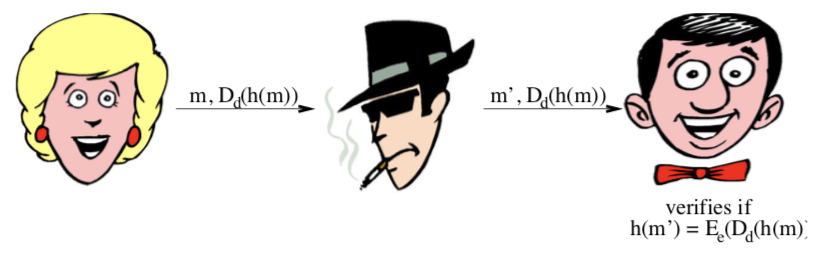
\includegraphics[scale=0.59]{sig}
\end{figure}
\noindent
Dunque le crittografie simmetrica/asimmetrica assicurano la confidenzialità distribuendo propriamente le chiavi. La crittografia asimmetrica semplifica la distribuzione delle chiavi (ma ha bisogno di un canale autenticato).\\
È importante implementare l'autenticazione dei messaggi, una volta che le chiavi sono state distribuite.



\chapter*{Public-Key Infrastructures}
\addcontentsline{toc}{chapter}{Public-Key Infrastructures}
È importante che esista un \textit{key management} per: distribuzione di chiavi crittografiche, creare un legame tra un'identità ed una chiave, generare, mantenere e revocare le chiavi (possono essere state rubato o scadute).\\\\
Un \textit{\textbf{PKI}} è un'infrastruttura che permette agli attori di riconoscere l'appartenenza di una \textit{public-key a qualcuno}.\\
Per fare parte del \textit{PKI}, un utente deve:
\begin{itemize}
	\item generare la sua coppia di chiavi privata/pubblica;
	\item inviare la sua chiave pubblica ad un \textbf{Certification Authority (CA)} affidabile per tutti;
	\item il \textbf{CA} verifica che l'utente sia colui che dice di essere e infine firma un \textit{certificato digitale} che assicura l'appartenenza di quella chiave pubblica al determinato utente.
	\item tutti gli altri utenti adesso possono verificare il certificato per ottenere la chiave pubblica di quell'utente.
\end{itemize}
\noindent
Le \textbf{componenti di un PKI} sono le seguenti:
\begin{itemize}
	\item \textbf{Certification Authority (CA)}: crea i certificati e li pubblica nella \textit{directory}; mantiene anche il \textit{Certificate Revocation List (CRL)} nella \textit{directory}.
	\item \textbf{Certificate Revocation List (CRL)}: interpellato per sapere se i certificati sono ancora validi. La \textit{CA} può anche revocare i certificati per motivi diversi. Si occupa del \textit{Key Recovery} in caso di smarrimento della chiave privata, di firma o di non ripudiazione (solitamente viene invalidata e creata una nuova).
	\item \textbf{Directory}: rende disponibili i certificati degli utenti (per identificarli univocamente) e il \textit{CRL};
	\item \textbf{Registration Authority (RA)}: si occupa del processo di registrazione degli utenti, assicurandone l'identità.
	\item \textbf{Clients}: gli utenti che si registrano e autenticano.
\end{itemize}
\noindent
Le \textit{PKI} possono essere \textbf{Open} (usate per compagnie e comunità) oppure \textbf{Closed} (limitate ad un gruppo di utenti).


\section*{Certificati}
\addcontentsline{toc}{section}{Certificati}
Un \textit{\textbf{certificato}} è un token che lega un'identità ad una chiave.\\
L'utente $C$ firma (con la sua chiave privata) un messaggio contenente la rappresentazione dell'identità di $Alice$, la corrispondente chiave pubblica ($PU_Alice$) e il \textit{timestamp} $T$:
$$ \mathcal{C}_{Alice} = M || E(PR_C, H(M)) \text{~~~dove~} M = \langle PU_{Alice}, Alice, T\rangle $$
\noindent
$B$ può verificare il certificato per ottenere la chiave pubblica di $Alice$ e accettarne la validità.\\
Tuttavia $B$ può conoscere la chiave pubblica di $C$ per validare il certificato.\\\\
Il problema è un altro adesso: come può essere convalidato il certificato dell'emittente?
\begin{itemize}
	\item costruire un albero gerarchico, con la chiave pubblica della radice conosciuta fuori dalla banda;
	\item oppure permettere una arrangiamento arbitrario affidandosi sulla conoscenza di ciascuno riguardo i certificatori.
\end{itemize}

\subsection*{X.509}
\addcontentsline{toc}{subsection}{X.509}
Per illustrare questi approcci, i certificati e le certificazioni, si prende come esempio il \textbf{X.509}.\\
\textit{\textbf{X.509}} è uno standard per l'utlizzo dei servizi di autenticazione. La struttura del certificato ed i protocolli di autenticazione in esso definiti sono utilizzati in molti contesti (\textit{IPSEC}, \textit{SSL/TLS}, \textit{SET} e \textit{S/MIME}).\\
Si basa sulla crittografia a chiave pubblica (raccomanda \textit{RSA}), funzioni di hash e firme digitali.
\begin{multicols}{2}
	\noindent
	Il cuore dello schema \textbf{X.509} è il certificato della chiave pubblica associato ad ogni utente. Viene creato dal \textit{CA} e messo nella \textit{directory} che garantisce un accesso semplice agli utenti per ottenere i certificati.
	\begin{itemize}
		\item \textit{Serial Number}: deve essere univoco in coppia al numero dell'emittente;
		\item \textit{Signature Algorithm Identifier}: identifica l'algoritmo, e ogni parametro utilizzato per firmare il certificato;
		\item \textit{Issuer Name}: il nome del CA che ha creato e firmato il certificato;
		\item \textit{Period of Validity}: scadenza del certificato;
		\item \textit{Subject Name}: nome dell'utente al quale il certificato si riferisce;
		\item \textit{Subject Public-Key Info}: identifica l'algoritmo, i parametri e la chiave pubblica dell'utente;
		\item \textit{Signature}: contiene l'hash code degli altri campi, criptati con la chiave privata del CA.
	\end{itemize}
\columnbreak
	\begin{figure}[H]
		\centering
		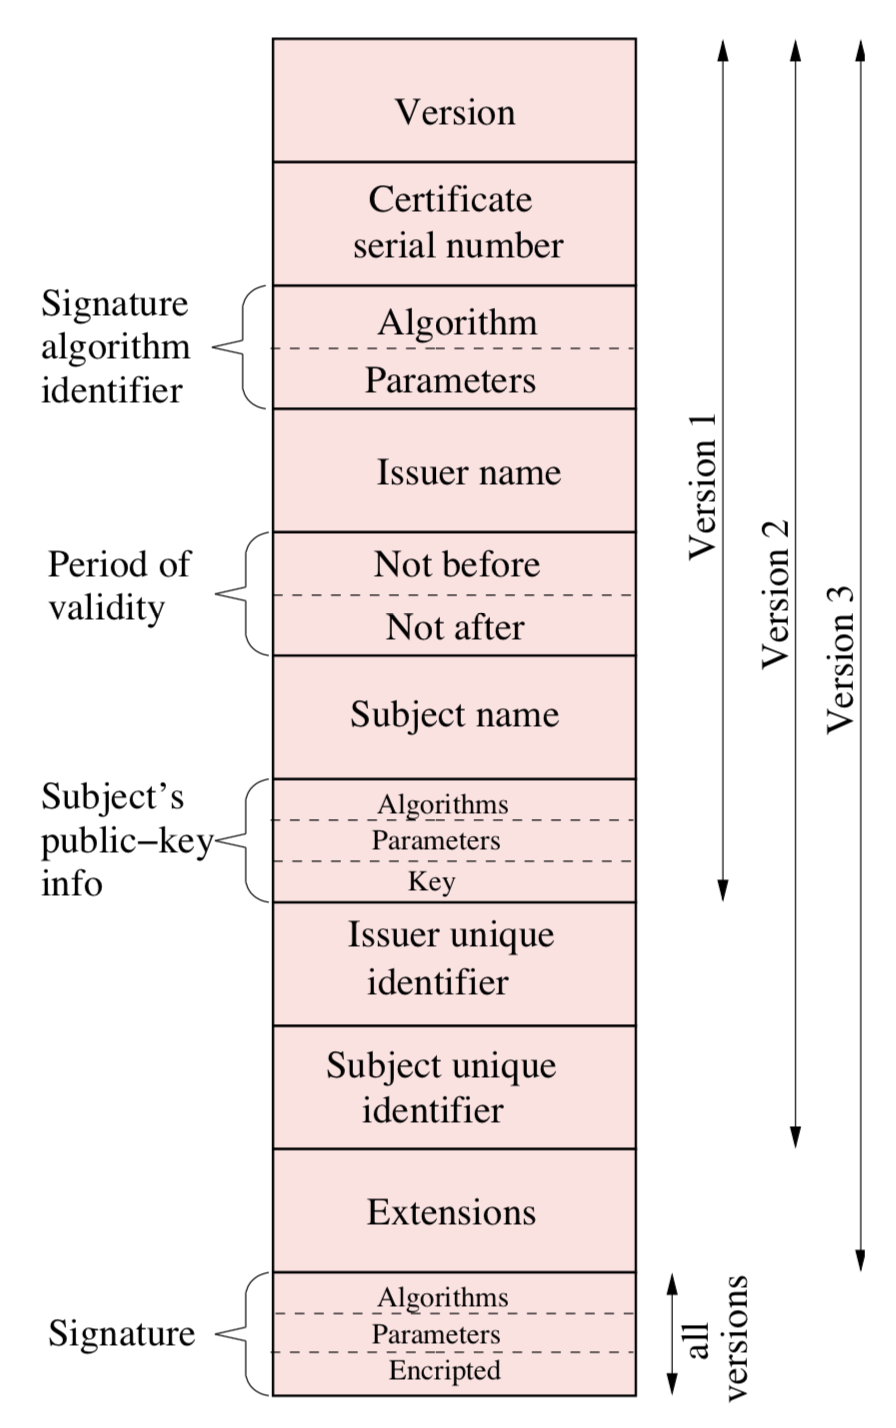
\includegraphics[scale=0.43]{x509}
	\end{figure}
\end{multicols}

\noindent
L'utente riceve $PU_{CA}$, decodifica il campo \textit{Signature}, computa l'hash del certificato e ne verifica la validità.


\section*{Trust Models}
\addcontentsline{toc}{section}{Trust Models}
Esistono diversi \textbf{\textit{Trust Models}} che dettano come gli utenti devono stabilire la validità di un certificato: \textit{Direct Trust}, \textit{Hierarchical Trust}, \textit{Web of Trust}.\\
\\
\textbf{Direct Trust}: se tutti gli utenti sono iscritti alla stessa \textit{CA}, c'è una fiducia comune verso di essa. Tutti i certificati si trovano nella stessa \textit{directory} per l'accesso da parte degli utenti che possono anche trasmetterseli (come in \textit{PGP}).\\
\\
\textbf{Hierarchical Trust}: per grandi community è più pratico avere più \textit{CA}, creando un \textbf{Trust Tree} che si estende da un numero di \textit{certificati radice}. Questi certificati possono certificare i certificati stessi oppure altri certificati che certificano altri certificati lungo la catena. La validità del \textit{certificato foglia} è verificata risalendo dal suo certificatore, ad altri certificatori, fino a quando non viene trovato un certificato radice attendibile.\\
\textit{\textbf{Cross Certification}}: se $A$ (con certificato nel CA $X_1$) vuole il certificato di $B$ (in $X_2$), può fare affidamento sul fatto che i due CA si siano scambiati le chiavi pubbliche. Dunque $A$ può ottenere il certificato di $B$ in una \textit{catena di certificati}.\\
Lo schema \textit{X.509} prevede appunto che i vari CA siano disposti secondo una \textit{gerarchia}.\\
\\
\textbf{Web of Trust}: comprende \textit{direct} e \textit{hierarchical trust}, aggiungendo l'idea che il trust sta nell'occhio dell'osservatore (visione del mondo reale) e che più informazioni sono migliori. Un certificato può essere \textit{trusted} direttamente oppure tramite una catena fino a risalire alla radice o ad un gruppo di \textit{introducers} (catene di fiducia).

\subsection*{Web of Trust: PGP}
\addcontentsline{toc}{subsection}{Web of Trust: PGP}
I certificati \textbf{PGP} differiscono da \textit{X.509} in alcuni punti importanti:
\begin{itemize}
	\item una chiave \textit{PGP} può avere molteplici firme (anche del proprietario) per aumentare la fiducia in quel certificato;
	\item ogni firma è una nozione di fiducia e le firme possono avere diversi livelli di fiducia (gli utenti agiscono in base a questo livello). Si tratta dunque di \textit{Reputation System} poiché non vi è l'autorità centrale.
\end{itemize}
\noindent
Nell'ambiente \textit{PGP}, ogni utente agisce come un CA firmando gli altri certificati. Firmando l'utente ne diventa un \textit{introducer}. Per definire inoltre se un certificato è valido è necessario conoscere uno dei firmatari oppure ricostruire una catena. Si stabilisce un \textit{web of trust}.\\
In \textit{PGP} i certificati indicano dunque un livello di fiducia che però può avere diversi significati per differenti firmatari.



\chapter*{Network Security and Internet Protocols}
\addcontentsline{toc}{chapter}{Network Security and Internet Protocols}
I protocolli sono essenziali per sviluppare servizi web poiché il \textit{mondo è distribuito}.
Un protocollo è un insieme di regole (convenzioni) che determinano l'ordine e le \textit{regole} per lo scambio di messaggi tra due o più attori; in breve è un \textit{algoritmo distribuito} che si occupa della comunicazione.\\
Un \textbf{protocollo di sicurezza} (oppure \textbf{crittografico}) usa meccanismi di crittografia per raggiungere obiettivi qualI: autenticazione degli utenti, scambio di chiavi, integrità $\dots$

\section*{Costruzione di un Protocollo per lo Sambio di Chiavi}
\addcontentsline{toc}{section}{Costruzione di un Protocollo per lo Sambio di Chiavi}
Per progettare un buon protocollo, bisogna stabilire l'architettura per le comunicazioni: si hanno due utenti (mittente $A$ e destinatario $B$) che vogliono creare una chiave di sessione in modo sicuro e protetto. Si dovranno appoggiare ad un server $S$ assunto come affidabile. Il server dovrà produrre una chiave di sessione segreta e autenticata da inviare (sempre in modo sicuro) ai due attori.\\
\textit{\textbf{Scopo finale del protocollo}}: $A$ e $B$ devono conoscere la chiave di sessione (e nessun altro tranne $S$!) e sapere che è stata appena generata (proprietà di \textit{freshness} contro i \textit{replay attack}).

\noindent
\textbf{\textit{\underline{Tentativo 1}}}: protocollo che si basa su 3 messaggi.
\begin{multicols}{2}
\begin{itemize}
		\item \textbf{Problemi}:
		La chiave viene passata in chiaro. Possiamo dichiarare che: l'avversario può intercettare tutti i messaggi.
\end{itemize}
	\columnbreak
	\begin{figure}[H]
		\centering
		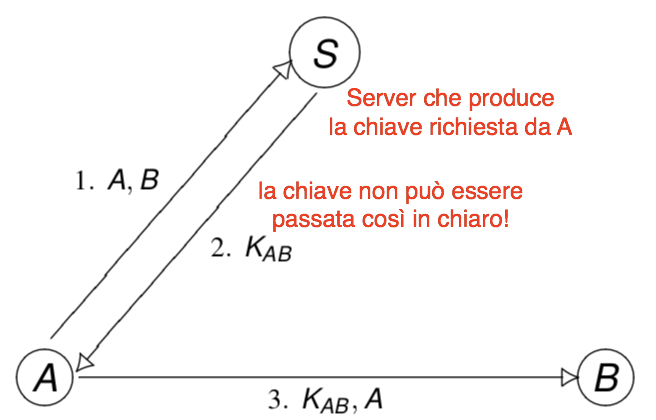
\includegraphics[scale=0.45]{attempt1}
	\end{figure} 
\end{multicols}

\noindent
\textbf{\textit{\underline{Tentativo 2}}}: il server $S$ manda le chiavi criptate per evitare che l'avversario possa ottenerle in chiaro.	
	\begin{multicols}{2}
		\begin{itemize}
			\item \textbf{Problemi}: l'avversario è in grado di alterare tutti i messaggi in transito usando qualsiasi informazione disponibile ed eseguirne il forwarding, forgiare e inserire nuovi messaggi (ha il controllo della rete).
	\end{itemize}

	\noindent
	Si possono verificare due casi di attacco in particolare:
	\begin{itemize}
		\item $B$ crede di condividere la chiave con $A$, ma in realtà la sta condividendo con $D$!
		\item $C$ altera i messaggi che $A$ manda ad $S$, così $S$ cripta i messaggi con la chiave di $C$. D'ora in poi $A$ pensa di spedire a $B$ ma in relatà sta comunicando con $C$.\\
		È un \textit{\textbf{masquerading attack}} perché $C$ impersonifica $B$ a causa della mancanza di \textbf{autenticazione}.\\
		In questo caso $C$ può essere un legittimo partecipante della rete (\textit{insider}) oppure un \textit{outsider}, o addirittura una combinazione di entrambi.
	\end{itemize}
\noindent
L'avversario può essere uno dei due attori \textit{(insider)} o una parte esterna \textit{(outsider)} o una combinazione delle due.
\columnbreak
	\begin{figure}[H]
		\centering
		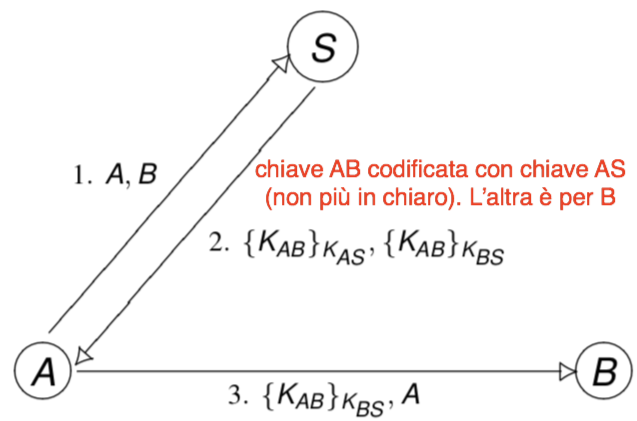
\includegraphics[scale=0.4]{attempt2}
	\end{figure}
	\begin{figure}[H]
		\centering
		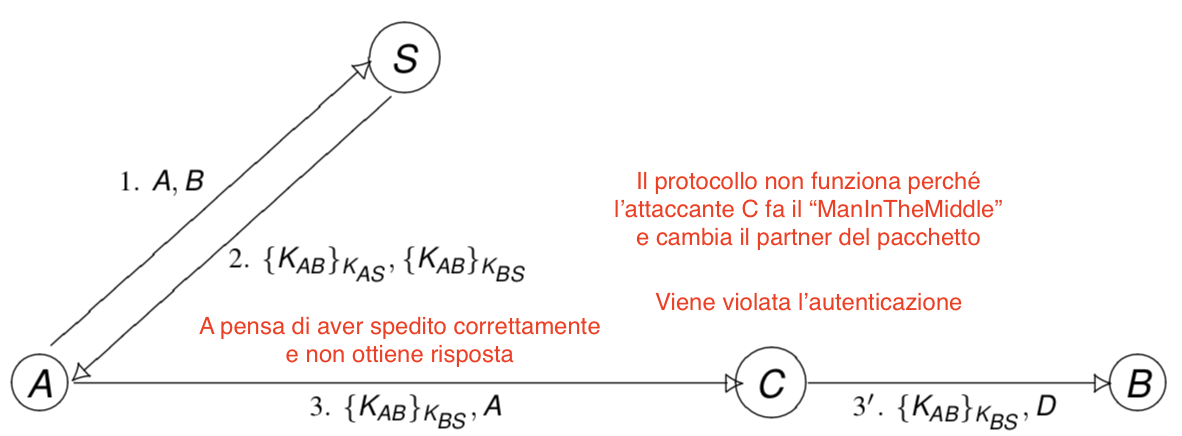
\includegraphics[scale=0.4]{problem1attempt2}
	\end{figure}
	\begin{figure}[H]
		\centering
		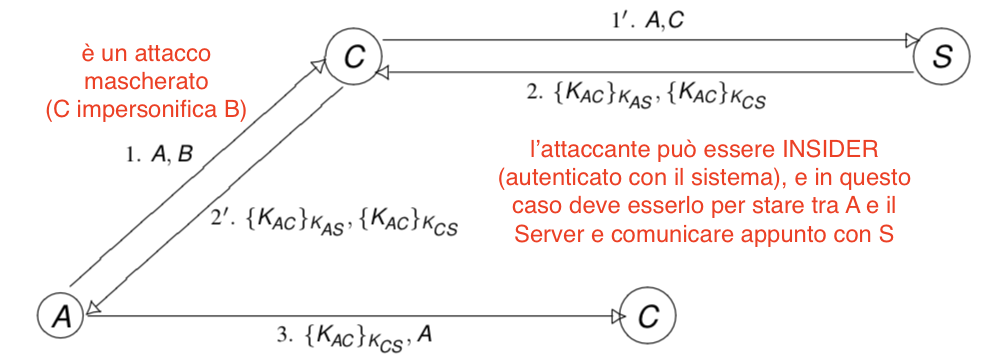
\includegraphics[scale=0.4]{problem2attempt2}
	\end{figure}
\end{multicols}
	
\noindent
\textbf{\textit{\underline{Tentativo 3}}}: il server $S$ manda le chiavi criptate indicando anche i nomi degli attori.
\begin{multicols}{1}
		\noindent
		Ora l'avversario non può origliare o alterare la conversazione tra le parti!
		\begin{itemize}
		\item \textbf{Problemi}: l'avversario può ottenere il valore della chiave di sessione $K_{AB}$ usata in un'esecuzione precedente del protocollo.
		\begin{itemize}
			\item $C$ intercetta i messaggi da $A$ ad $S$
			\item \textbf{Replay attack}: $K'_{AB}$ è una chiave vecchia usata da $A$ e $B$ in una sessione precedente. Viene meno la \textbf{freshness} della chiave. Per ovviare al problema si usano i \textbf{nonce}.
		\end{itemize}
	\end{itemize}
	\columnbreak
	\begin{figure}[H]
		\centering
		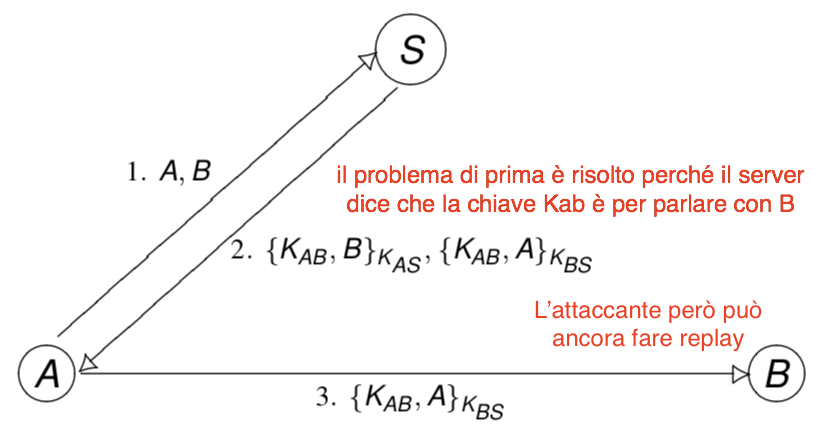
\includegraphics[scale=0.5]{attempt3}
	\end{figure}
	\begin{figure}[H]
		\centering
		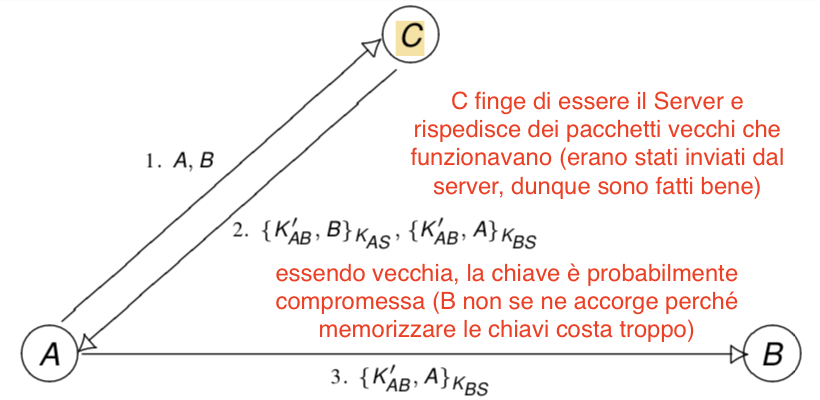
\includegraphics[scale=0.5]{problem1attempt3}
	\end{figure}
\end{multicols}
	
\begin{multicols}{2}
	\noindent
	\textbf{\textit{\underline{Tentativo 4}}}: noto come \textbf{Needham e Schroeder} ($1978$).
	\begin{itemize}
		\item È attualmente uno dei protocolli più conosciuti ma è vulnerabile all'attaco fatto da \textit{Denning e Sacco}.\\
		Si basa sui \textbf{nonce}\textit{ (number used only once)}, cioè un valore generato randomicamente da uno degli utenti per dimostrare che il messaggio è nuovo (lo riceverà anche nella risposta).
		\item \textbf{Problemi}: se il protocollo abortisce, $A$ non è sicuro che $B$ abbia ricevuto o meno la chiave (è necessaria la \textbf{key confirmation}).
		\begin{itemize}
			\item $C$, mascherato come $A$ può inviare una vecchia chiave a $B$; nel frattempo $A$, non ricevendo risposte da $B$, abortisce il protocollo. Mentre $B$ continua la conversazione con $C$ utilizzando una chiave corrotta (senza sapere che la chiave è corrotta e che dall'altra parte non vi è realmente $A$).
		\end{itemize}
	\end{itemize}
\columnbreak
	\begin{figure}[H]
		\centering
		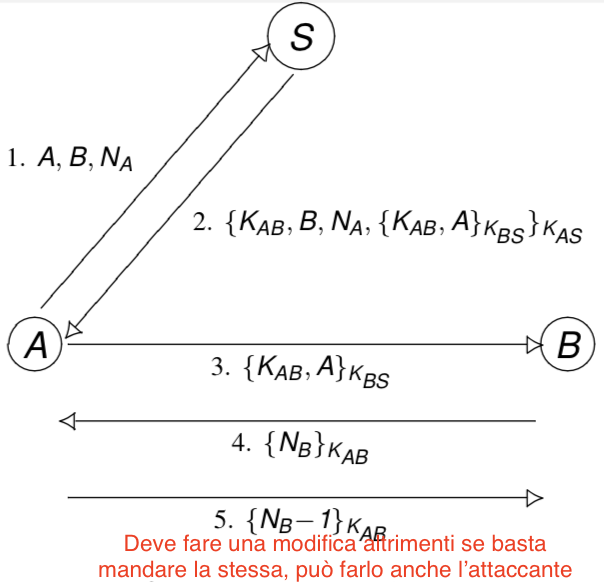
\includegraphics[scale=0.55]{attempt4}
	\end{figure}
	\begin{figure}[H]
		\centering
		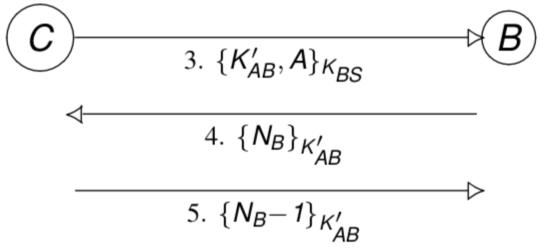
\includegraphics[scale=0.55]{problem1attempt4}
	\end{figure}
\end{multicols}

\begin{multicols}{2}
	\noindent
	\textbf{\textit{\underline{Tentativo 5}}}: \textit{\textbf{Kerberos}}.
	\begin{itemize}
		\item L'\textit{initiator} è $B$ che manda il suo \textit{nonce} e identità ad $A$; quest'ultimo aggiunge il suo \textit{nonce} e lo manda al server per ricevere la chiave.\\
		Infine $A$ manda la chiave, la sua identità e il \textit{nonce} di $B$ al mittente (criptato con la sua chiave).\\
		La proprietà di \textbf{key confirmation} è raggiunta sapendo che il messaggio $4$ può essere creato solamente conoscendo $K_{AB}$.
	\end{itemize}
	\columnbreak
	\begin{figure}[H]
		\centering
		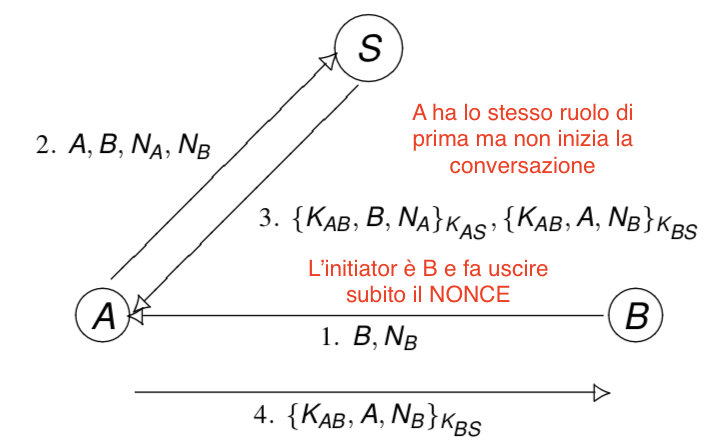
\includegraphics[scale=0.5]{attempt5}
	\end{figure}
\end{multicols}
\noindent
Alla fine del protocollo conclusivo, nessuno dei due attori ha la certezza che l'altro abbia ricevuto $K_{AB}$.\\
\textbf{Questo protocollo evita tutti gli attacchi visti in precedenza}. È comunque azzardato affermare che esso sia sicuro.\\
La sicurezza di un protocollo si può definire in relazione agli obiettivi da raggiungere (da formalizzare con esso).


\newpage
\section*{Il Protocollo di Needham-Schroeder a Chiave Pubblica (NSPK)}
\addcontentsline{toc}{section}{Il Protocollo di Needham-Schroeder a Chiave Pubblica (NSPK)}
Il \textit{protocollo NSPK} (nato nel $1970$) ha i seguenti obiettivi:
\begin{multicols}{2}
	\begin{itemize}
		\item \textit{mutua autenticazione} legando messaggi e mittente;
		\item Assicurare che i messaggi siano recenti (\textit{timeliness});
		\item garantire la \textit{secrecy} di alcuni elementi (chiavi).
	\end{itemize}
\columnbreak
	\begin{figure}[H]
		\centering
		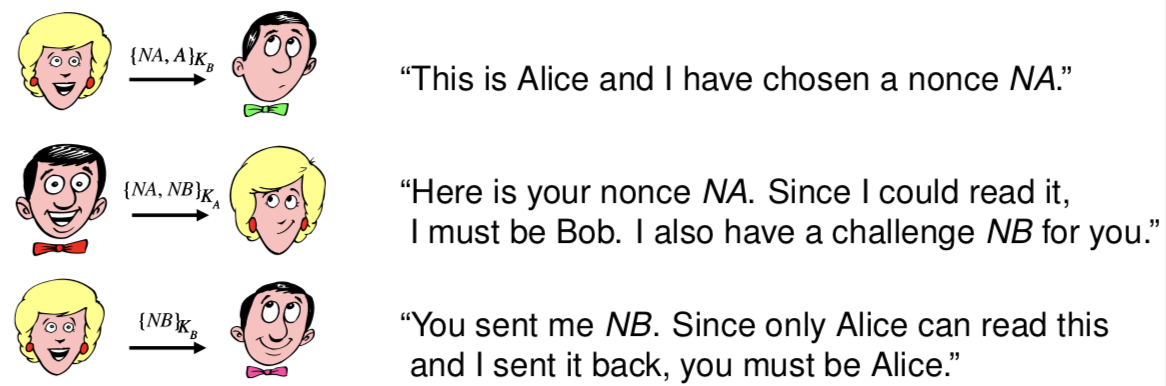
\includegraphics[scale=0.45]{NSPK}
	\end{figure}
\end{multicols}

\begin{multicols}{2}
	\noindent
	\textbf{MiTM di tipo masquerading attack}
	\\\\
	Ciò è dovuto all'assenza del \textbf{binding} al passo $2$:\\
	$B \longrightarrow A\ :\ \{ NA, NB,$ \textbf{$B$}$\}$.\\\\
	È molto importante legare al \textit{nonce} il nome del mittente, altrimenti il protocollo non è sicuro.\\
	La versione migliorata è il protocollo \textbf{NSL}.
\columnbreak
	\begin{figure}[H]
		\centering
		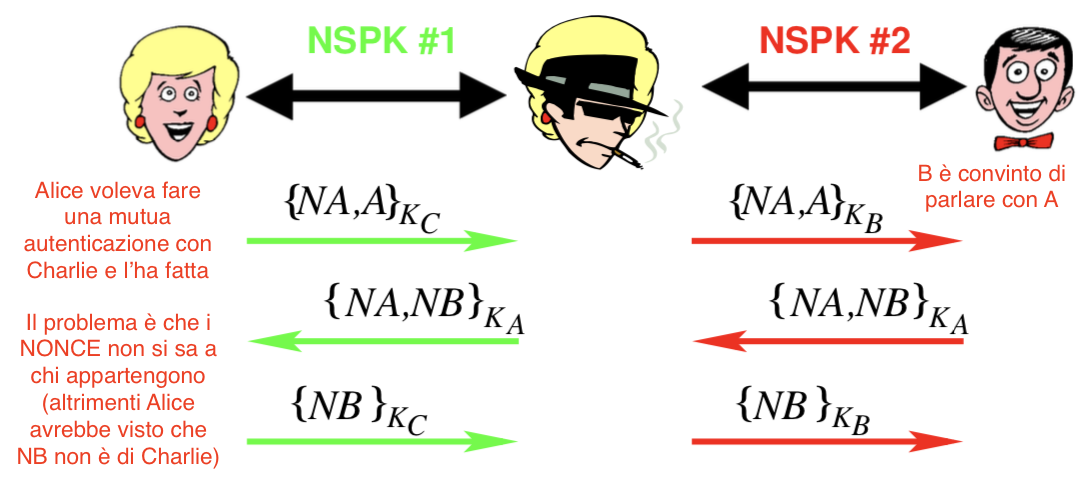
\includegraphics[scale=0.46]{mitmnspk}
	\end{figure}
\end{multicols}


\section*{Il Protocollo NSL (Needham-Schroeder-Lowe)}
\addcontentsline{toc}{section}{Il Protocollo NSL (Needham-Schroeder-Lowe)}
\begin{multicols}{2}
	\noindent
	Se consideriamo \textbf{autenticazione} e \textbf{segretezza}, questo protocollo è sicuro.\\\\
	Considerando invece l'\textbf{aliveness} degli attori (se $B$ volesse solamente sapere se $A$ è \textit{alive}), quello presentato in figura può essere considerato un attacco!
\columnbreak
	\begin{figure}[H]
		\centering
		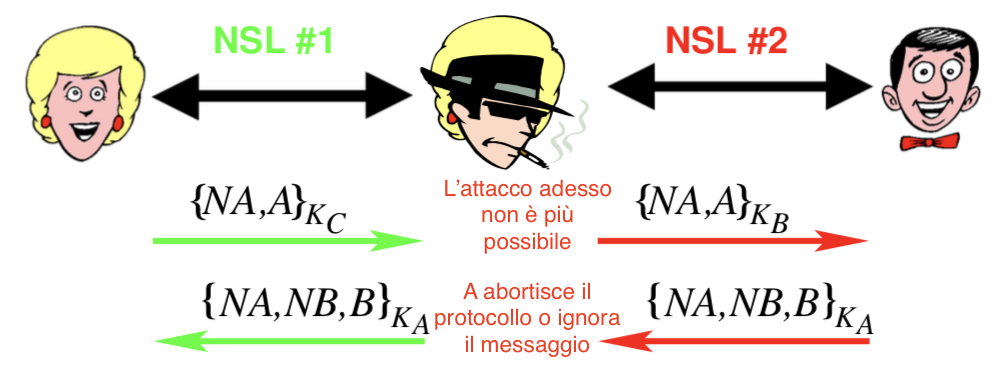
\includegraphics[scale=0.45]{nsl}
	\end{figure}
\end{multicols}

\begin{multicols}{3}
\noindent
\textbf{\textit{Type-Flaw \& Oracle Attack}}
\begin{figure}[H]
	\centering
	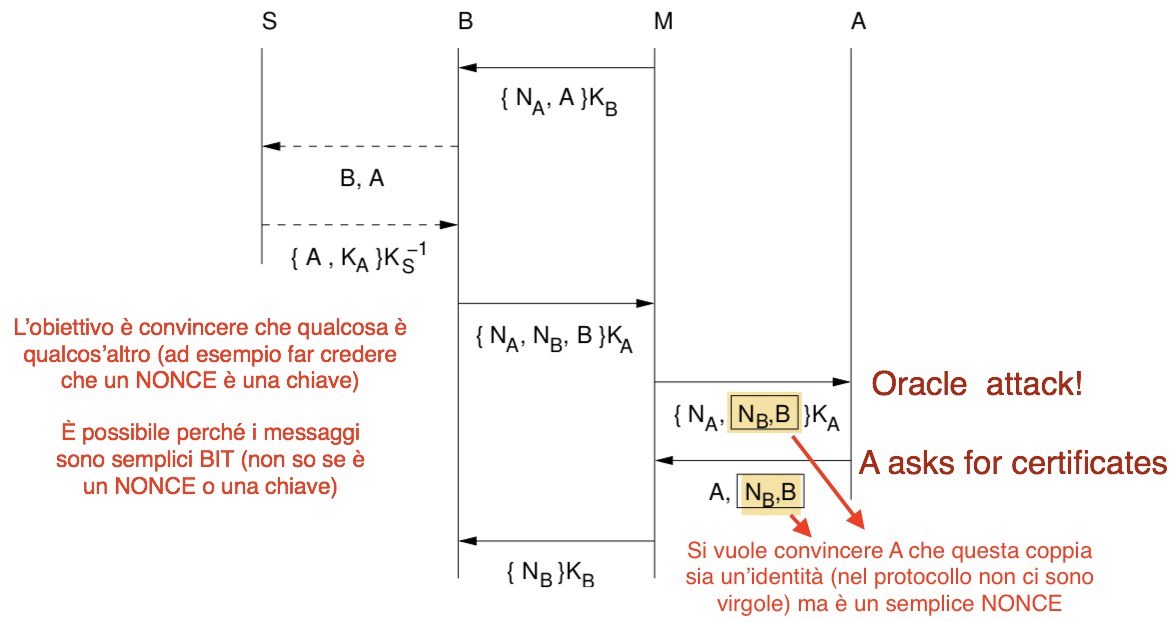
\includegraphics[scale=0.6]{lowetypeflaw}
\end{figure}
\columnbreak
~\\

\columnbreak
~\\\\
\noindent
Un'\textbf{altra soluzione} consiste nello scambio dei \textit{nonce} firmati con la chiave privata del mittente.\\\\
\textbf{M1.} $A \rightarrow B: \{ [N_A, A]_{K_A^{-1}} \}_{K_B}$\\
\textbf{M2.} $B \rightarrow A: \{ N_A, [N_B]_{K_B^{-1}} \}_{K_A}$\\
\textbf{M3.} $A \rightarrow B: \{ [N_B]_{K_A^{-1}} \}_{K_B}$
\end{multicols}

\section*{Tipi di Attacco}
\addcontentsline{toc}{section}{Tipi di Attacco}
\begin{itemize}
	\item \textbf{MitM attack}: $A \leftrightarrow Z \leftrightarrow B $, come in DH (bisogna aggiungere uno scambio di ID con messaggi firmati).
	\item \textbf{Replay attack}: riutilizzare parti di messaggi vecchi (o vecchie chiavi);
	\item \textbf{Masquerading attack}: im personificare un'altro attore. Può avvenire in due modi:
		\begin{itemize}
			\item $Z$ forgia un indirizzo sorgente (nei protocolli di rete)
			\item $Z$ convince altri attori che la chiave pubblica di $A$ è $K_{Z}$ (per fare \textit{spoofing attack});
		\end{itemize}
	\item \textbf{Reflection attack}: reinvio di informazioni al mittente;
	\item \textbf{Oracle attack}: uso delle risposte previste dal protocollo come strumenti di codifica/decodifica;
	\item \textbf{Type flaw attack}: sostituzione di un campo con un'altra informazione che verrà interpretata dal ricevente in un modo favorevole all'attaccante.
\end{itemize}


\section*{Il Protocollo di Otway-Rees}
\addcontentsline{toc}{section}{Il Protocollo di Otway-Rees}
\begin{multicols}{2}
	\noindent
	È un protocollo \textit{server-based} per distribuzione di chiavi autenticate (con \textit{key freshness}) ma senza autenticazione dell'entità coinvolta o \textit{key confirmation}.\\
	Le chiavi del server sono note e $I$ è l'identificatore del protocollo utilizzato (un intero).
\columnbreak
	\begin{figure}[H]
		\centering
		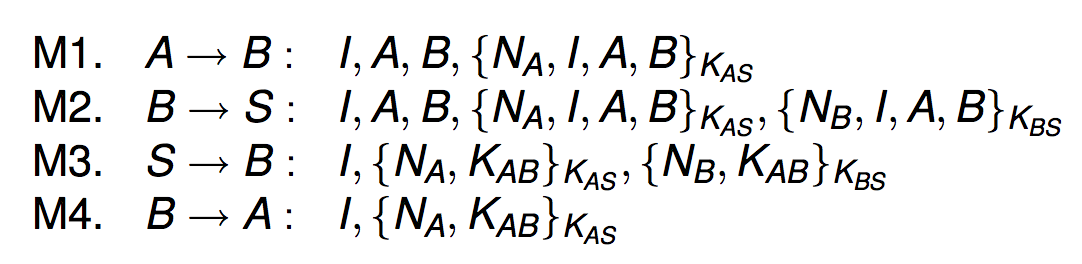
\includegraphics[scale=0.5]{otway-rees}
	\end{figure}
\end{multicols}
\begin{multicols}{2}
\noindent
\textbf{Vulnerabilità}:\\
Assumiamo che $\vert\{I,A,B\}\vert = \vert\{K_{AB}\}\vert$,\\
cioé se $I$ è 32 bit, $A$ e $B$ sono 16 bit, allora $K_{AB}$ è 64 bit.
\begin{figure}[H]
	\centering
	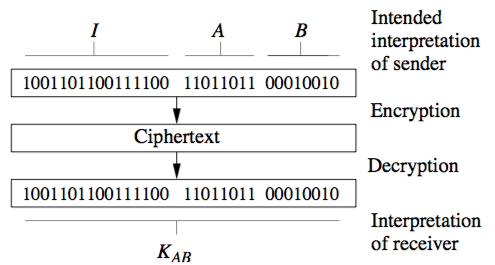
\includegraphics[scale=0.7]{otway-reestypeflaw}
\end{figure}
\end{multicols}
\noindent
\textbf{Segretezza e autenticazione violate!}
\begin{multicols}{2}
\begin{itemize}
		\item \textbf{Attacco 1} (\textit{Reflection/type flaw}): l'attaccante $Z$ fa un \textit{replay} delle parti del messaggio 1 e 4 (omettendo gli step 2 e 3);\\
		Ora $A$ vede $N_{A}$ e accetta ${I,A,B}$ come \textit{session key}!
\end{itemize}
	\columnbreak
	\begin{figure}[H]
		\centering
		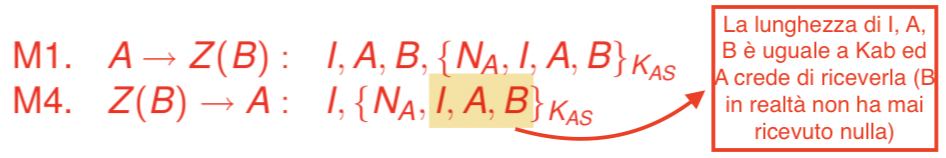
\includegraphics[scale=0.5]{otway-reestypeflaw2}
	\end{figure}
\end{multicols}

\begin{multicols}{2}
\begin{itemize}
	\item \textbf{Attacco 2}: Z può giocare il ruolo di $S$ in M2 e M3 riflettendo il messaggio M2 a  $B$.\\
	Adesso $A$ e $B$ accettano la chiave sbagliata e $Z$ può decriptare le loro comunicazioni.\\
	Falliscono autenticazione e \textit{secrecy}.
\end{itemize}
\columnbreak
	\begin{figure}[H]
		\centering
		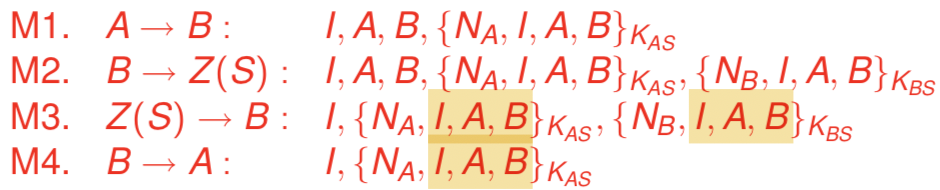
\includegraphics[scale=0.5]{otway-reesattack2}
	\end{figure}
\end{multicols} 


\section*{Il Protocollo di Andrew Secure RPC}
\addcontentsline{toc}{section}{Il Protocollo di Andrew Secure RPC}
\begin{multicols}{2}
	\noindent
	Con questo protocollo si vuole scambiare una chiave condivisa, autenticata, fresh tra due attori che condividono già una chiave simmetrica. Il protocollo stabilisce una chiave di sessione $K'_{AB}$ e un nonce $N'_{B}$ per una sessione futura.
\columnbreak
	\begin{figure}[H]
		\centering
		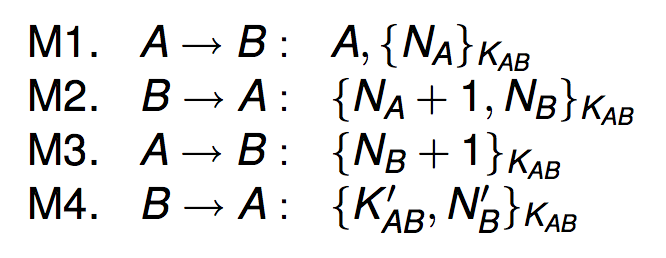
\includegraphics[scale=0.4]{andrewsecurerpc}
	\end{figure}
\end{multicols}

\begin{multicols}{2}
	~\\\\
\textbf{Vulnerabilità}: \textit{Type-flaw attack}
\\\\
Assumiamo che nonce e chiavi siano rappresentati da sequenze di bit della stessa lunghezza (es: 64 bit).
\columnbreak
	\begin{figure}[H]
		\centering
		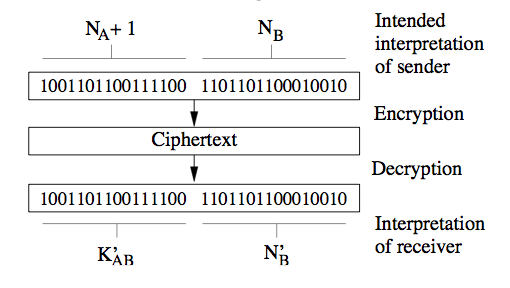
\includegraphics[scale=0.8]{andrewsecurerpctypeflaw}
	\end{figure}
\end{multicols}

\begin{multicols}{2}
	\noindent
	$Z$ può registrare M2, intercettare M3 e mandare M2 come replay di M4. $A$ a questo punto è forzato ad accettare $N_{A} +1$ come chiave, la chiave \textbf{non è autenticata}. L'attacco tuttavia \textit{non viola la segretezza}.
\columnbreak
	\begin{figure}[H]
		\centering
		\includegraphics[scale=0.43]{andrewsecurerpctypeflawattack}
	\end{figure}
\end{multicols}


\section*{Scambio delle chiavi con CA (Denning \& Sacco)}
\addcontentsline{toc}{section}{Scambio delle chiavi con CA (Denning \& Sacco)}
\begin{multicols}{3}
	\noindent
	$B$ è certo che sta comunicando con $A$ perché decripta con $K_A$ che è legata al certificato $C_A$. Sa che il messaggio è destinato a lui perché è criptato con la sua chiave pubblica.
\columnbreak
	\begin{itemize}
		\item $K_A^{-1}$ chiave privata di $A$;
		\item $C_A, C_B$ certificati per $A$ e $B$;
		\item $T_A$ \textit{timestamp} generato da $A$, limita l'uso della \textit{session key}.
	\end{itemize}
\columnbreak
	\begin{figure}[H]
		\centering
		\includegraphics[scale=0.75]{denningsacco}
	\end{figure}
\end{multicols}

\noindent
\textbf{Vulnerabilità}: \textit{MitM masquerading attack}
\begin{multicols}{2}
\noindent
$B$ crede che l'ultimo messaggio sia spedito da $A$, di conseguenza andrà ad utilizzare $K_{AZ}$, permettendo a $Z$ di intercettare tutto.\\\\
Per difendersi da questo tipo di attacco \textit{MitM} è necessario esplicitare i nomi degli attori nell'ultimo passo.
\columnbreak
	\begin{figure}[H]
		\centering
		\includegraphics[scale=0.5]{denningsaccomitm}
	\end{figure}
	\begin{figure}[H]
		\centering
		\includegraphics[scale=0.5]{denningsaccomitm2}
	\end{figure}
\end{multicols}


\section*{Esempi di Attacchi}
\addcontentsline{toc}{section}{Esempi di Attacchi}
\begin{multicols}{2}
\begin{itemize}
	\item \textbf{Binding attack}
	\begin{figure}[H]
		\centering
		\includegraphics[scale=0.48]{bindingattack}
	\end{figure}
\end{itemize}
\columnbreak
\begin{itemize}
	\item \textbf{Parallel session attack}
	\begin{figure}[H]
		\centering
		\includegraphics[scale=0.48]{parallelsession}
	\end{figure}
\end{itemize}
\end{multicols}
\begin{multicols}{2}
\begin{itemize}
	\item \textbf{Replay attack}
	\begin{figure}[H]
		\centering
		\includegraphics[scale=0.55]{replayattack}
	\end{figure}
\end{itemize}
\columnbreak
\begin{itemize}
	\item \textit{\textbf{Trasformazioni crittografiche} (con 2 notazioni)}
	\begin{itemize}
		\item $\{ M \}_K$ indica che $M$ è criptato con chiave $K$, garantendo \textbf{confidentiality} poiché può essere letto solo da chi possiede la chiave $K^{-1}$.
		\item $[ M ]_K$ indica che $M$ è criptato con chiave $K$ attraverso una trasformazione \textit{one-way}, garantendo \textbf{data integrity} con l'origine. Il messaggio può essere visto da chi possiede la chiave di decriptazione $K^{-1}$ e la chiave $K$ di verifica che ne controlla l'integrità (ritorna \textit{yes} se non ci sono state violazioni).\\\\
		Rappresentabile anche con $\{ M \}_{K_1}^{K_2}$ denotando che $M$ è criptato con chiave $K_1$ e protetto nella \textit{data-integrity} con chiave di verifica $K_2$.
	\end{itemize}
\end{itemize}
\end{multicols}



\chapter*{Kerberos, SSL, IPSec}
\addcontentsline{toc}{chapter}{Kerberos, SSL, IPSec}
\section*{Kerberos}
\addcontentsline{toc}{section}{Kerberos}
\textbf{Protocollo per} l'\textbf{autenticazione} in ambienti aperti e distribuiti. In principio doveva contenere altre due componenti: \textit{accounting} (logging) e \textit{audit} (registrare ciò che accade), ma non sono mai state implementate.\\
Prenderemo in esame la versione $IV$ (1989), tutt'ora utilizzata da molti siti.\\
I \textbf{requisiti} di questo protocollo sono i seguenti::
\begin{itemize}
	\item \textbf{Sicuro}: un attaccante non deve essere in grado di impersonificare un altro utente (no \textit{masquerading}/\textit{spoofing}).
	\item \textbf{Affidabile}: deve supportare un architettura distribuita, dove un sistema può eseguire il backup di un altro.
	\item \textbf{Trasparente}: ogni utente deve usare le proprie credenziali per ottenere i servizi richiesti e non deve avere conoscenza di ciò che accade più a basso livello (\textit{single sign-on}, cioè si registra una volta sola).
	\item \textbf{Scalabile}: il sistema deve supportare un gran numero di utenti e server (architettura modulare e distribuita).
\end{itemize}
\begin{multicols}{2}
	\noindent
	Si basa approssimativamente sul protocollo \textit{Needham-Schroeder Shared-Key}, utilizzando il \textbf{timestamp} al posto dei \textit{nonce} per garantire la \textit{freshness} delle chiavi.\\
	Il \textit{timestamp} viene creato in base all'orologio di $T$, dunque le altre macchine devono essere sincronizzate (un attaccante dovrebbe desincronizzarle).
\columnbreak
	\begin{figure}[H]
		\centering
		\includegraphics[scale=0.45]{taut}
	\end{figure}
\end{multicols}
\begin{multicols}{2}
	\begin{itemize}
		\item \textbf{Autenticazione} utilizza il $KAS$ (\textit{Kerberos Authentication Server}) per fornire un tiket da portare al \textit{TGS};
		\item \textbf{Autorizzazione} utilizza il $TGS$ (\textit{Ticket Granting Server}) che verifica il primo ticket e ne fornisce un altro per utilizzare la risorsa richiesta;
		\item \textbf{Access Control}, dove il server verifica i biglietti del \textit{TGS} prima di fornire la risorsa richiesta.
	\end{itemize}
\columnbreak
	\begin{figure}[H]
		\centering
		\includegraphics[scale=0.55]{kerberos}
	\end{figure}
\end{multicols}


\subsection*{Fase di Autenticazione}
\begin{multicols}{2}
	\begin{itemize}
		\item $A$ effettua il login e richiede una risorsa.
		\item $KAS$ accede al database e manda ad $A$ la chiave di sessione $K_{A, TGS}$ e il ticket criptato \textit{AuthTicket}.
		\item $A$ scrive la password sulla workstation per decriptare il risultato (salvato per sessione).
	\end{itemize}
\columnbreak
	\begin{itemize}
		\item Quando $K_{A,TGS}$ scade, $A$ non è più loggato.
		\item $K_{A,TGS}$: chiave di sessione che dura alcune ore (dipende dall'applicazione);
		\item $K_{AS}$ è derivata dalla password utente. Entrambe le chiavi devono essere registrate nel database.
	\end{itemize}
\end{multicols}
\begin{figure}[H]
	\centering
	\includegraphics[scale=0.7]{kerbauthphase}
\end{figure}


\subsection*{Fase di Autorizzazione}
\begin{itemize}
	\item $A$ presenta al $TGS$ il \textbf{ticket di autenticazione} (\textit{AuthTicket}) del passo 2. Presenta un \textbf{autenticatore} della durata di pochi secondi per evitare \textit{replay attacks} (memorizzate anche dal server per evitare \textit{immediate replay});
	\item $TGS$ risponde con una nuova chiave di sessione $K_{AB}$ (con la durata di pochi minuti) ed un nuovo ticket \textbf{ServTicket}. $K_{B, TGS}$ è la chiave condivisa tra \textit{TGS} e la risorsa in rete.
	\item il secondo ticket ha una durata più breve rispetto a quello di autenticazione perché $A$ può interagire spesso con il \textit{TGS} durante una giornata (mentre è loggato).
\end{itemize}
\begin{figure}[H]
	\centering
	\includegraphics[scale=0.5]{kerbauthorphase2}
\end{figure}


\subsection*{Fase di servizio}
\begin{multicols}{2}
	\begin{itemize}
		\item $A$ presenta il ticket del passo 4 con un \textbf{nuovo autenticatore} per poter accedere alla risorsa $B$;
		\item $B$ assicura che la richiesta è stata ricevuta ($A$ può essere messo in attesa se la risorsa è occupata).
	\end{itemize}
\columnbreak
	\begin{figure}[H]
		\centering
		\includegraphics[scale=0.6]{kerbservicephase}
	\end{figure}
\end{multicols}


\subsection*{Scalabilità - Multiple Realms/Kerberi}
\begin{multicols}{2}
	\noindent
	Un \textit{\textbf{realm}} è definito da un \textit{Kerberos server}.\\
	Le grandi reti devono necessariamente essere suddivise in \textit{realms} amministrativi.\\\\
	\textit{Kerberos} supporta anche i \textbf{protocolli inter-realm}, cioé permette agli utenti di un \textit{realm} di utilizzare risorse situate in un altro \textit{realm}.
	\begin{itemize}
		\item i server sono registrati tra loro;
		\item se $A$ vuole accedere alla risorsa $B$ in un altro \textit{realm}, il \textit{TGS} del \textit{realm} di $A$ fornisce i ticket per accedere al \textit{TGS} nel \textit{realm} di $B$.
		\item l'estensione del protocollo è semplice perché vengono aggiunti solamente due nuovi passi.
		\item il problema riguarda la complessità: per $n$ \textit{realms}, nella versione $IV$ il problema di distribuzione delle chiavi è $O(n^{2})$.
	\end{itemize}
\columnbreak
	\begin{figure}[H]
		\centering
		\includegraphics[scale=0.8]{kerberi}
	\end{figure}
\end{multicols}

\subsection*{Limitazioni di \textit{Kerberos IV}}
\begin{itemize}
	\item \textbf{M1}: la crittografia non serve, però un attaccante può inondare il $KAS$ (Denial of Service);
	\item \textbf{M2}: la doppia cifratura è ridondante (rimossa in \textit{Kerberos V}): \[ KAS \rightarrow A: A,\{K_{A,TGS}, TGS, \tau_{1} \}_{K_{AS}},\{A, TGS, K_{A,TGS}, \tau_{1} \}_{K_{KAS, TGS}} \]
	\item si basa su \textbf{clock} sincronizzati e non compromessi. Se l'host è compromesso, anche il \textit{clock} può essere compromesso, facilitando i \textbf{replay attack}.
\end{itemize}
\noindent
Alcune di queste limitazioni sono ancora presenti in \textit{Kerberos V} che viene utilizzato come nuovo standard.


\newpage
\section*{SSL (Secure Socket Layer)}
\addcontentsline{toc}{section}{SSL (Secure Socket Layer)}
Garantisce comunicazioni \textit{end-to-end} sicure in presenza di un attaccante, usato specialmente nella navigazione web.\\
Agisce tra client (es. \textit{web browser}) e server (es. \textit{website}). Usa i certificati digitali per verificare le identità degli attori e le loro chiavi pubbliche (spesso solamente il server è autenticato). Opera al di sopra del \textit{livello di trasporto}.
\begin{multicols}{2}
	\noindent
	Usa le chiavi pubbliche per stabilire un segreto condiviso.\\
	\textit{\textbf{SSL}} si basa su due protocolli:
	\begin{itemize}
		\item \textit{Handshake}: usa la crittografia a chiave pubblica per stabilire chiavi condivise tra client e server;
		\item \textit{Record}: usa la chiave segreta stabilita nella modalità \textit{Handshake} per proteggere confidenzialità, integrità e autenticità dei dati scambiati tra client e server.
	\end{itemize}
\columnbreak
	\begin{figure}[H]
		\centering
		\includegraphics[scale=0.6]{sslrecap}
	\end{figure}
\end{multicols}


\subsection*{Fasi del Protocollo}
\begin{multicols}{2}
\begin{itemize}
	\item \textit{\textbf{Hello}}
	\begin{figure}[H]
		\centering
		\includegraphics[scale=0.6]{sslhello}
	\end{figure}
	\begin{itemize}
		\item $A$ identifica il client, nella pratica si utilizza l'indirizzo IP;
		\item $Sid$ è l'identificatore di sessione;
		\item $P_{a}$ è la lista delle preferenze di $A$ per criptazione e compressione, cioé i protocolli che utilizza (es. \textit{Diffie-Hellmann} per la signature, \textit{RSA} per lo scambio delle chiavi);
		\item $P_{b}$ è il protocollo con la versione maggiore, supportata da entrambi (si basa su $P_{a}$); entrambi inviati non protetti e, se la chiave privata è compromessa, l'attaccante ottiene ciò che vuole.
	\end{itemize}
\end{itemize}
\columnbreak
\begin{itemize}
	\item \textit{\textbf{Server Certificate}}
	\begin{figure}[H]
		\centering
		\includegraphics[scale=0.6]{sslservercertificate}
	\end{figure}
\begin{itemize}
	\item \textit{Certificato}: \textbf{X.509v3} firmato da una terza parte affidabile; la fiducia si basa tutta sul certificato verificato dal browser.
	\item il server può richiedere il certificato del client, ma accade molto raramente.
\end{itemize}
\end{itemize}
\end{multicols}

\begin{multicols}{2}
\begin{itemize}
	\item \textit{\textbf{Client exchange}}
	\begin{figure}[H]
		\centering
		\includegraphics[scale=0.55]{sslclientexchange}
	\end{figure}
	\begin{itemize}
		\item $PMS$ è un \textbf{pre-master secret} usato per computare un \textbf{master secret} $M$; viene utilizzato per generare varie chiavi attraverso il metodo $P_a$ e $P_b$ concordato (viene inviato criptato con la chiave pubblica del server se utilizzano \textit{RSA}).\\
		Es: $M = PRF(PMS, N_{a}, N_{b})$ con $PRF$ funzione pseudo-random (costruita dal MAC).
	\end{itemize}
\end{itemize}
\columnbreak
\begin{itemize}
	\item \textit{\textbf{Finish}}
	\begin{figure}[H]
		\centering
		\includegraphics[scale=0.55]{sslfinish}
	\end{figure}
	\begin{itemize}
		\item \textit{Finished} è un hash dei messaggi precedentemente inviati (garantendo l'integrità degli oggetti). Previene \textbf{downgrade} e \textbf{MitM attack}.
		\item \textit{clientK} e \textit{serverK} sono chiavi simmetriche per cifratura/decifratura di client e server; entrambe generate da $N_a$, $N_b$ e $M$, cioé dal $PMS$.\\
		I messaggi seguenti saranno inviati utilizzando queste chiavi di cifratura.
	\end{itemize}
\end{itemize}
\end{multicols}

\noindent
\textbf{Vulnerabilità}: \textit{Rollback attack}
\begin{itemize}
	\item Un attaccante potrebbe interporsi tra il client e il server, modificando la versione richiesta dal client. Questo perchè il \textit{server adatta il protocollo in base alle richieste del client}. Utlizzando la versione $2.0$ di \textit{SSL}, non è inclusa la fase \textit{Finish} dei messaggi (\textbf{rollback attack} possibile perché $P_a$ è passato in chiaro).\\
	\item I nuovi protocolli vengono introdotti perché quelli vecchi non sono più sicuri; però le nuove versioni devono essere \textit{backward-}compatibili poiché non tutti effettuano gli upgrade.
	\item Una risoluzione possibile, nella fase di \textbf{client key exchange}, è inviare: ~~~$ C \rightarrow S: \{version_{c}, secret_{c} \}_{PK_{s}}$\\
	In questo modo, se l'\textbf{hello} viene \textbf{alterato}, il server capisce la modifica.
\end{itemize}

\noindent
\textbf{SSL Striping}\\
L'\textit{\textbf{icona}} del \textit{\textbf{lucchetto}} nella barra di ricerca del browser viene mostrata quando la pagina è sicura da attacchi di rete.
\begin{figure}[H]
	\centering
	\includegraphics[scale=0.7]{sslstriping}
\end{figure}
\begin{itemize}
	\item Nei siti in cui si passa da HTTP a HTTPS mediante javascript (\textit{mixed content}), un attaccante può instaurare una connessione HTTPS con il server e HTTP con il client, o HTTPS con il client iniettando il proprio certificato.\\ \textbf{N.B}: l'attacco non dovrebbe funzionare se il sito supporta HSTS (High-Strict Transport Security).
	\item  possono essere errori di implementazione degli sviluppatori (le banche servono tutti i contenuti in \textit{HTTPS}).\\
	\textbf{\textit{N.B.}}: i contenuti, nel secondo caso, sono serviti con lo stesso protocollo del resto della pagina.
\end{itemize}
\begin{multicols}{2}
\begin{figure}[H]
	\centering
	\includegraphics[scale=0.5]{scr1}
\end{figure}
\columnbreak
\begin{figure}[H]
	\centering
	\includegraphics[scale=0.5]{scr2}
\end{figure}
\end{multicols}

\noindent
\textbf{Phishing}\\
Un altro enorme \textbf{problema} nell'ambito della sicurezza di rete è il \textbf{\textit{phishing}}, nonostante esista \textit{SSL}.\\
Vengono spedite moltissime mail, spacciandosi per aziende note, che richiedono di inserire dati sensibili all'interno di pagine non protette (ma l'utente inesperto non se ne accorge perché magari non distingue \textit{HTTP} da \textit{HTTPS}).\\
Una \textbf{soluzione} può essere la combinazione di \textit{SSL} e \textit{GSM} (telefoni cellulari), inviando un \textbf{TAN} \textit{Transaction Authentication Number} via sms per l'autenticazione.\\
Non è troppo sicuro poiché il numero del client è salvato all'interno del server: rischio di \textit{MitM attack}.

\begin{figure}[H]
	\centering
	\includegraphics[scale=0.9]{layers}
\end{figure}


\newpage
\section*{IPSec}
\addcontentsline{toc}{section}{IPSec}
Il protocollo internet (\textit{IP}) non è sicuro: inventato agli albori di internet, quando la sicurezza non era un problema.
\begin{multicols}{2}
	\noindent
\textit{IP Security} (\textbf{\textit{IPSec}}) dovrebbe colmare tutte le lacune lasciate dal protocollo IP (sia \textit{IPv4} che \textit{IPv6}), tra cui:
\begin{itemize}
	\item \textit{spoofing della sorgente};
	\item \textit{replay dei pacchetti};
	\item \textit{confidenzialità}: cifratura dei dati;
	\item \textit{integrità dei dati}: tutti i router calcolano il checksum oppure l'hash dei dati;
	\item \textit{autenticazione}: firma dei certificati.
\end{itemize}
\columnbreak
\begin{figure}[H]
	\centering
	\includegraphics[scale=0.5]{ipsecscenario}
\end{figure}
\end{multicols}
\noindent
Fornisce un canale sicuro a tutte le applicazioni per cifratura e autenticazione del traffico. Ha inoltre la capacità di filtrare, basandosi su una policy, come se ci fosse un \textit{firewall} tra le due entità. È installato nei sistemi operativi (sicurezza end-to-end), nei gateway di sicurezza (router, firewall); viene utilizzato anche per implementare le \textit{VPN (Virtual Private Network}, macchine remote che condividono un metodo di comunicazione come se appartenessero alla stessa rete).\\\\
\textit{IPSec} è un protocollo molto complesso e, di conseguenza, molto difficile da attaccare:
\begin{itemize}
	\item \textbf{\textit{Authentication Header (AH)}}: protegge integrità e autenticità dei datagrammi IP (non la confidenzialità);
	\item \textbf{\textit{Encapsulating Security Payload (ESP)}}: protegge la confidenzialità e, opzionalmente, l'integrità;
	\item \textbf{\textit{Key Management (IKE)}}: \textit{Internet Key Exchange Protocol} per la creazione del tunnel IPSec.
\end{itemize}
\noindent
\textit{\textbf{Security Association} (SA)}: è una relazione unidirezionale tra mittente e destinatario. Ne servono 2 per definire i servizi di sicurezza, specificando: \textit{authentication algorithm (AH)}, \textit{encryption algorithm (ESP)}, chiavi, vita delle chiavi, vita della \textit{SA}, modalità del protocollo (\textit{tunnel} oppure \textit{transport}). La \textit{SA} viene stabilita utilizzando \textit{IKE} (o altri protocolli).

\subsection*{Transport \& Tunnel Mode}
\textbf{IPSec} può lavorare in \textbf{due modalità}:
\begin{multicols}{2}
\begin{itemize}
	\item \textit{\textbf{Transport mode}}:
		\begin{itemize}
			\item l'header IPSec viene inserito nel pacchetto IP;
			\item viene criptato il payload del datagramma IP (nessun nuovo pacchetto);
			\item Non si  nasconde l'identità della sorgente;
			\item utile per le reti in cui l'incremento della dimensione dei pacchetti può creare problemi;
			\item Usato nelle VPN remote-access.
		\end{itemize}
	\end{itemize}
\columnbreak
	\begin{itemize}
		\item \textit{\textbf{Tunnel mode}}:
		\begin{itemize}
			\item viene criptato l'intero datagramma IP, diventando poi parte dei dati di un nuovo pacchetto IP più grande;
			\item Nasconde l'identità della sorgente;
			\item Usato nelle VPN site-to-site.
		\end{itemize}
	\end{itemize}
\end{multicols}
\begin{figure}[H]
	\centering
	\includegraphics[scale=0.55]{ipsectransporttunnel}
\end{figure}


\subsubsection*{Authentication Header (AH)}
\begin{multicols}{2}
	\noindent
	Viene aggiunto un nuovo header tra il livello 3 e 4 (IP e TCP), fornendo al destinatario abbastanza informazioni per identificare la \textit{SA}.\\
	\textit{AH} garantisce l'integrità e protegge parte dell'header IP.\\
	Il \textit{sequence number} è inizializzato a zero e incrementato dal mittente per ogni pacchetto. In questo modo il destinatario può ordinarli ed eliminare i duplicati.\\
	\\
	Il MAC del pacchetto è inserito in \textit{Authentication Data}.
\columnbreak
	\begin{figure}[H]
		\centering
		\includegraphics[scale=0.75]{ahstructure}
	\end{figure}
\end{multicols}

\noindent
\textbf{Garantisce autenticazione}
\begin{multicols}{2}
\begin{itemize}
	\item \textit{\textbf{Transport mode}}:
		\begin{figure}[H]
			\centering
			\includegraphics[scale=0.5]{ahtransportmode}
		\end{figure}
		\begin{itemize}
			\item \textit{AH} inserito dopo l'header IP e prima del payload;
			\item MAC dell'intero pacchetto (eccetto campi mutabili);
			\item garantisce una protezione end-to-end tra i sistemi abilitati \textit{IPSec}.
		\end{itemize}
\columnbreak
	\item \textit{\textbf{Tunnel mode}}:
		\begin{figure}[H]
			\centering
			\includegraphics[scale=0.5]{ahtunnelmode}
		\end{figure}
		\begin{itemize}
			\item autenticato l'intero pacchetto, con un nuovo IP header;
			\item l'header più interno contiene l'indirizzo dell'ultima sorgente e destinazione;
			\item anche il nuovo header è protetto e può contenere diversi indirizzi IP (es. firewall o gateway di sicurezza).
		\end{itemize}
\end{itemize}
\end{multicols}

\subsubsection*{Encapsulating Security Payload (ESP)}
\begin{figure}[H]
	\centering
	\includegraphics[scale=0.8]{espstructure}
\end{figure}
\begin{multicols}{2}
\begin{itemize}
	\item Transport mode:
	\begin{figure}[H]
		\centering
		\includegraphics[scale=0.7]{esptransportmode}
	\end{figure}
		\begin{itemize}
			\item Cripta solo il \textit{payload} di ogni pacchetto, senza toccare l'header;
			\item usato per end-to-end encryption tra host che supportano IPSec.
		\end{itemize}
	\begin{figure}[H]
		\centering
		\includegraphics[scale=0.53]{tras}
	\end{figure}
\columnbreak
	\item Tunnel mode:
		\begin{figure}[H]
			\centering
			\includegraphics[scale=0.7]{esptunnelmode}
		\end{figure}
		\begin{itemize}
			\item l'intero datagramma IP viene incapsulato nell'ESP. \textit{Il vecchio header} ed il \textit{payload} vengono criptati (e opzionalmente autenticati);
			\item modalità usata per VPN
		\end{itemize}
	\begin{figure}[H]
		\centering
		\includegraphics[scale=0.33]{tunn}
	\end{figure}
\end{itemize}
\end{multicols}


\subsection*{Servizi IPSec}
\begin{figure}[H]
	\centering
	\includegraphics[scale=0.7]{recapipsec}
\end{figure}
\begin{figure}[H]
	\centering
	\includegraphics[scale=0.65]{recapipsec2}
\end{figure}


\subsection*{IKE}
\addcontentsline{toc}{subsection}{IKE}
\textit{\textbf{IKE}} è la base fondante per l'handshake in \textit{IPSec} e si è evoluto da diversi protocolli basati su \textit{Diffie-Hellmann}:
\begin{itemize}
	\item \textit{ISAKMP} (\textit{Internet Security Association and Key Management}): framework per stabilire associazioni sicure e le relative chiavi crittografiche (però era sprovvisto di meccanismi di autenticazione);
	\item \textit{Oakley}: protocolli di key agreement.
\end{itemize}
\textit{IKE} si basa molto su \textit{Diffie-Hellman}, sfruttando la proprietà della \textbf{PFS} (\textit{perfect forward secrecy}): un attaccante che intercetta la conversazione non può decriptarla neanche in seguito grazie alla \textit{chiave di sessione temporanea}, non derivabile dalle informazioni del nodo dopo la chiusura della sessione.\\
Non stabilisce solo le chiavi ma anche le (\textit{SA}). È un protocollo molto flessibile ma complesso; esso è composto da:
\begin{itemize}
	\item \textbf{\textit{Fase 1}}: negoziazione tra due parti di una \textit{Security Association} (\textit{SA}) attraverso le \textit{master keys} per stabilire il materiale di codifica condiviso.\\
	\textit{Master keys}: chiavi simmetriche segrete pre-condivise, chiave pubblica di cifratura, o chiave pubblica di firma.
	\item \textbf{\textit{Fase 2}}: la \textit{SA} viene usata per creare \textit{SA} figlie per autenticare e cifrare le nuove comunicazioni.
\end{itemize}
\begin{figure}[H]
	\centering
	\includegraphics[scale=0.35]{ikeroadmap}
\end{figure}

\subsection*{Fase 1}
La fase $1$ offre due modalità (entrambe risultanti nella \textit{SA} desiderata):
\begin{itemize}
	\item \textbf{\textit{Main Mode}}: 6 messaggi tra $I$ e $R$. Offre protezione dell'identità e flessibilità nella negoziazione dei parametri.
	\item \textbf{\textit{Aggressive Mode}}: più veloce ma meno protezione. Si basa su 3 messaggi scambiati. Non ha protezione dell'identità tranne quando viene usata la crittografia a chiave pubblica per l'autenticazione.
\end{itemize}
Ogni modalità ha 4 varianti, basati sul metodo di autenticazione (chiave condivisa, firme digitali e due varianti a chiave pubblica). Prendiamo in esame la \textbf{Main Mode}:
\begin{multicols}{2}
	\begin{figure}[H]
		\centering
		\includegraphics[scale=0.62]{ikefase1mainmode}
	\end{figure}
\columnbreak
	\begin{figure}[H]
		\centering
		\includegraphics[scale=0.54]{ikefase1mainmodeschematico}
	\end{figure}
\end{multicols}

\begin{multicols}{2}
\subsubsection*{A chiave condivisa}
\begin{figure}[H]
	\centering
	\includegraphics[scale=0.7]{ikefase1mainmodemessaggi}
\end{figure}
\begin{itemize}
	\item \textbf{1}: $ISA_{I}$ (ISAKMP SA per $I$) è il numero di proposte crittografiche con una lista di algoritmi; Viene inviato un \textit{cookie} per evitare \textit{DoS/Clogging} in caso di elevato numero di richieste dallo stesso IP.
	\item \textbf{2}: $ISA_{R}$ (ISAKMP SA per $R$) è il numero di proposte crittografiche accettate e gli algoritmi scelti; ritorna anche un altro \textit{cookie}, oltre a quello del mittente.
	\item \textbf{3} e \textbf{4}: contengono le half-key per DH, i nonce di $I$ ed $R$ ed i rispettivi \textit{cookie}.
	\item \textbf{5} e \textbf{6}: sono crittografati con la chiave generata da \textit{Diffie-Hellman}. $AUTH_{I}$ e $AUTH_{R}$ sono l'autenticazione dei messaggi precedenti attraverso un MAC o una firma.
\end{itemize}
\columnbreak
\subsubsection*{A chiave pubblica}
\begin{figure}[H]
	\centering
	\includegraphics[scale=0.5]{ikefase1mainmodechiavepubblica}
\end{figure}

\subsubsection*{Negoziazione fallita}
\begin{figure}[H]
	\centering
	\includegraphics[scale=0.8]{fail}
	\caption*{$R$ non supporta nessuna delle proposte di $I$.}
\end{figure}
\end{multicols}

\newpage
L'\textbf{Aggressive Mode} si basa sui seguenti 3 messaggi:
\begin{itemize}
	\item il mittente propone la SA, inizia lo scambio DH, manda un numero pseudorandomico e la propria identità IKE;
	\item il destinatario accetta la SA, autentica il mittente, manda un numero pseudorandomico, la sua identità IKE e, se possiede un certificato, lo manda;
	\item il mittente autentica il destinatario, conferma lo scambio e, se possiede un certificato, lo manda.
\end{itemize}


\subsection*{Fase 2 (Quick mode)}
Tutto il traffico viene criptato utilizzando la \textit{ISAKMP Security Association} poiché è stato creato un canale sicuro. Ogni negoziazione \textit{quick mode} risulta in due \textit{IPSec Security Association} per mettere in sicurezza i dati nel tunnel IPSec.
\begin{itemize}
	\item Vengono scelti algoritmi di cifratura e autenticazione per i dati trasmessi.
	\item SI scegli il protocollo di sicurezza (AH oppure ESP).
	\item Crea e aggiorna le chiavi sfruttando la PFS di Diffie-Hellman.
\end{itemize}
\begin{multicols}{2}
	\begin{figure}[H]
		\centering
		\includegraphics[scale=0.5]{ikefase2roadmap}
	\end{figure}
\columnbreak
	\begin{figure}[H]
		\centering
		\includegraphics[scale=0.45]{ikefase2quickmodemessaggi}
	\end{figure}
\end{multicols}



\chapter*{Intrusion Detection System}
\addcontentsline{toc}{chapter}{Intrusion Detection System}
Un problema significativo per sistemi di rete sono gli \textit{\textbf{accessi indesiderati}} o \textit{\textbf{ostili}}.\\
Ci sono diverse classi di \textit{\textbf{intruders}} (oppure \textit{hackers/crackers}):
\begin{itemize}
	\item \textit{\textbf{Masquerader}}: un individuo non autorizzato a utilizzare il computer (\textit{outsider});
	\item \textit{\textbf{Misfeasor}}: utente legittimato che accede in maniera non autorizzata a dati, risorse o abusa dei privilegi (\textit{insider});
	\item \textit{\textbf{Clandestine User}}: individuo che prende il controllo del supervisore del sistema per eludere \textit{access control} e \textit{audit}.
\end{itemize}
\noindent
Gli \textit{intruders} possono essere \textbf{benigni} (esplorano la rete e consuma risorse rallentando le performance) oppure \textbf{maligni} (accedono ai dati modificandoli e corrompendo il sistema). \textit{IDS/IPS/VPN} possono essere d'aiuto.\\
\\
Il \textbf{comportamento di un hacker} segue dei passi ben precisi:
\begin{multicols}{2}
	\begin{itemize}
		\item sceglie un target attraverso dei tools di \textit{IP lookup};
		\item mappa la rete per trovare servizi accessibili;
		\item identifica i servizi potenzialmente vulnerabili;
		\item può eseguire un \textit{brute force attack} per ottenere delle password;
	\end{itemize}
\columnbreak
	\begin{itemize}
		\item può installare nel target dei tool per l'amministrazione remota;
		\item può attende che l'admin effettui il login per catturarne la password;
		\item utilizza la password per accedere al resto della rete.
	\end{itemize}
\end{multicols}

\noindent
\textit{\textbf{Criminal Enterprise}}: gruppi di hacker organizzati con un obiettivo preciso. Quando penetrano agiscono in velocità ed escono. Per questo motivo i dati sensibili hanno bisogno di una maggiore sicurezza. Agiscono seguendo dei passi:
\begin{multicols}{2}
	\begin{itemize}
		\item commettono pochissimi errori.
		\item sfruttano le porte vulnerabili;
		\item usano degli \textit{sniffers} per catturare password;
	\end{itemize}
\columnbreak
	\begin{itemize}
		\item usano \textit{trojan horse} nascosti per lasciare un'entrata nascosta da cui rientrare;
		\item agiscono velocemente ed in maniera precisa per rendere le loro attività difficili da individuare;
	\end{itemize}
\end{multicols}

\noindent
\textit{\textbf{Insider Attacks}}: tra i più difficili da rilevare e prevenire. Gli impiegati hanno accesso e conoscono il sistema. Possono avere diversi motivi per fare danni (es. licenziamenti). \textit{IDS/IPS} possono aiutare ma hanno bisogno di: meno privilegi, monitoraggio dei logs, strong authentication e processi di terminazione per bloccare gli accessi. Agisce come segue:
\begin{multicols}{2}
	\begin{itemize}
		\item crea account di rete per sè e per i loro amici;
		\item accede ad account e applicazioni che normalmente non utilizza per lavori quotidiani;
		\item conduce conversazioni furtive;
	\end{itemize}
\columnbreak
	\begin{itemize}
		\item visita siti web che si rivolgono a impiegati scontenti;
		\item effettua molti download e copie di file;
		\item accede alla rete durante le ore di riposo.
	\end{itemize}
\end{multicols}

\noindent
\textit{\textbf{Intrusion Techniques}}: ottenere l'accesso e/o incrementare i privilegi nel sistema. Sfrutta le vulnerabilità del sistema o di alcuni software. L'obiettivo principale è quasi sempre ottenere delle password per impersonificare un altro utente.
\begin{itemize}
	\item \textbf{Password Guessing}: l'attaccante conosce un login (da email, pagina web $\dots$) e prova a indovinare la password da informazioni sull'utente. Il successo dipende dalla password scelta dall'utente (spesso poco sicura).
	\item \textbf{Password Capture}: spiare l'immissione da parte dell'utente, utlizzare un \textit{trojan horse}, monitoraggio di network login non sicuro, estrarre informazioni dalla cronologia web e dalla cache.
\end{itemize}

\noindent
\textit{\textbf{Intrusion Detection}}: è inevitabile avere delle falle nel sistema di sicurezza, però è necessario rilevare le intrusioni nel sistema, bloccarle e raccogliere informazioni per migliorare la sicurezza. Un intruso agisce in modo diverso dagli altri utenti legittimati all'interno del sistema; è comunque molto difficile da identificare.
\newpage
\noindent
Esistono principalmente due approcci per la \textit{Intrusion Detection}:
\begin{itemize}
	\item \textit{\textbf{Statistical Anomaly Detection} (profile of the user)}: definisce i comportamente aspettati da un utente e verifica se ci sono deviziani da esso. Definisce anche una soglia di rilevamento (\textit{threshold detection}) per contare le occorrenze di un evento nel tempo e valutare se è un valore ragionevole oppure c'è un'anomalia.
	\item \textit{\textbf{Rule-based Detection} (profile of the attack)}: definisce i modelli dell'attacco per il rilevamento di anomalie; si ricercano inoltre dei comportamenti sospetti (\textit{penetration identification}). Osserva gli eventi nel sistema e applica i modelli (di attacchi noti) per decidere se un'attività è sospetta o meno.
	\item \textit{Audit Records}: sono un tool fondamentale per l'\textit{intrusion detection} e possono essere nativi oppure specifici (costo maggiore ma sono creati specificatamente per collezionare le informazioni desiderate).
\end{itemize}
\noindent
Un \textit{Intrusion Detection System} deve rilevare una elevata percentuale di intrusioni con il minor numero di falsi allarmi; se rileva poche intrusioni non è sicuro, se ci sono troppi falsi allarmi viene ignorato (perdita di tempo).\\
\\
\textit{\textbf{Distributed Intrusion Detection}}: è una difesa più effettiva che si occupa di più sistemi connessi ad una rete.\\
\textit{Problemi}: diversi formati degli \textit{audit record}, integrità e confidenzialità dei dati in rete, architettura centralizzata o meno.
\begin{multicols}{2}
	\begin{figure}[H]
		\centering
		\includegraphics[scale=0.4]{dis}
	\end{figure}
\columnbreak
\begin{figure}[H]
	\centering
	\includegraphics[scale=0.42]{disagent}
\end{figure}
\end{multicols}
\begin{multicols}{2}
	\noindent
	\textit{\textbf{Honeypots}}: sistemi serviti come esche per adescare l'attaccante; sembrano interessanti per le informazioni che cerca un attaccante. Lo incoraggiano a restare nel sistema per catturare informazioni sulle sue attività.
	\begin{itemize}
		\item \textit{Location 1}: situato all'esterno, non può attirare attaccanti interni, soprattutto se il firewall filtra il traffico in entrambe le direzioni.
		\item \textit{Location 2}: situato nella rete  di servizi esterni (\textit{DMZ, Demilitarized Zone}); i sistemi in quella rete sono sicuri però il firewall blocca alcuni accessi a quella \textit{network area}. Perciò spesso il firewall deve aprire maggiormente al traffico, aumentando i rischi.
		\item \textit{Location 3}: situato all'interno, può rilevare attacchi interni e anche firewall configurati male che collegano internet alla rete interna; se l'\textit{honeypot} è comopromesso, ci possono essere attacchi interni.
	\end{itemize}
\columnbreak
	\begin{figure}[H]
		\centering
		\includegraphics[scale=0.55]{honeypot}
	\end{figure}
\end{multicols}

\noindent
\textit{\textbf{Password Management}}: è la prima linea di difesa contro gli intrusi. Utilizzano il \textit{login} (per determinare i privilegi dell'utente) e la \textit{password} per identificarsi. Quest'ultima viene salvata criptata (con \textit{DES} o funzioni di hash crittografico).\\
Gli utenti solitamente generano password deboli; è necessario educarli riguardo l'importanza di una buona password.\\
Le password più sicure sono quelle generate dal computer: difficili, mai utilizzate da altri, complesse da memorizzare.
\textit{\textbf{Proactive Checking}}: permette all'utente di scegliere la password ma il sistema verifica se è accettabile (compara con un dizionario di password cattive; usa algoritmi per rilevare scelte deboli).



\chapter*{Firewall}
\addcontentsline{toc}{chapter}{Firewall}
\begin{multicols}{2}
	\noindent
	Tutte le organizzazioni, e agenzie governative vogliono essere connesse alla rete e interconnettere tutte le reti.\\
	Non è semplice mettere in sicurezza tutti i sistemi dell'organizzazione: di solito si utilizzano i \textit{\textbf{Firewall}} per avere una difesa perimetrale con un singolo \textit{choke point}.
\columnbreak
	\begin{figure}[H]
		\centering
		\includegraphics[scale=0.52]{firewall}
	\end{figure}
\end{multicols}

\noindent
Il \textit{Firewall} è un \textit{choke point} per il controllo e monitoraggio che interconnette reti con diverso livello di \textit{trust}. Impone restrizioni ai servizi di rete, consentendo solo il traffico autorizzato: effettua un controllo sugli accessi e può fornire allarmi riguardo comportamenti anormali (fornisce una \textit{NAT}). Deve essere impenetrabile.\\
\\
\textbf{Limitazioni}: non può proteggere da attacchi che lo bypassano (\textit{trusted organization and services}), attacchi interni, accessia via \textit{WLAN} e malware importati da altri dispositivi.\\
\\
\textit{\textbf{Tipi di Firewall}}:
\begin{itemize}
	\item \textit{\textbf{Packet Filters}}: esamina ogni pacchetto IP e ne consente o meno l'accesso alla rete seguendo le regole (controlla \textit{source/dest IP}, protocollo IP $\dots$). Limita l'accesso ai servizi (porte) e segue una \textit{policy} di default (ciò che non è espressamente permesso è proibito, ciò che non è espressamente proibito è permesso).\\
	\textit{\textbf{Attacchi ai Packet Filters}}:
	\begin{itemize}
		\item \textit{Spoofing degli indirizzi IP}: servono filtri per pacchetti con indirizzo sorgente falso (l'intruso trasmette un pacchetto dall'esterno con IP di origine di un host interno ed arriva sull'interfaccia esterna del Firewall).
		\item \textit{Source routing attack}: l'attaccante imposta una \textit{route} diversa da quella di default per evitare controlli di sicurezza; è necessario bloccare i pacchetti con \textit{source routed}.
		\item \textit{Tiny fragment attack}: le informazioni vengono suddivise in tanti piccoli pacchetti poiché, solitamente, il firewall controlla solo il primo; è necessario accettare pacchetti con una dimensione minima.
	\end{itemize}
	\item \textit{\textbf{Stateful Packet Filters}}: i \textit{packet filters} tradizionali non esaminano i pacchetti fino agli strati più alti. Gli \textit{stateful packet filters} esaminano ogni pacchetto IP tenendo traccia della sessione client-server e controllano la validità di ciascun pacchetto. Mantiene una directory con ogni connessione TCP aperta e permette solo il traffico di queste.
	\item \textit{\textbf{Application Level Gateway} (or Proxy)}: ha piena conoscenza del protocollo. L'utente avanza la richiesta al proxy che la valida, la esegue e ritorna all'utente il risultato della richiesta. Controlla il traffico a livello applicativo.\\
	È necessario separare i proxy per ogni servizio: alcuni lo supportano naturalmente, altri sono più problematici.\\
	Lo svantaggio è l'\textit{overhead} poiché deve monitorare il traffico in entrambe le direzioni.
	\item \textit{\textbf{Circuit Level Gateway}}: trasmette due connessioni TCP. Impone la sicurezza limitando quali connessioni sono ammesse. Una volta create, trasmette il traffico senza analizzare il contenuto. Viene usato quando gli utenti interni fidati vogliono effettuare una connessione esterna.\\
	L'utente esterno deve collegarsi al \textit{SOCKS (SOCKet Secure)} nella porta 1080 (solitamente) e inviare la richiesta. I pacchetti vengono instradati tra client e server, passando dal proxy.
\end{itemize}
\noindent
\textit{\textbf{Bastion Host}}: si pone tra la connessione internet pubblica e la rete privata, filtrando tutti i contenuti scambiati: in caso di attacco il sistema lo blocca impedendo l'accesso alla rete locale. Questo computer ospita generalmente una singola applicazione (es. \textit{circuit/application level gateway}), mentre tutti gli altri servizi non essenziali vengono rimossi o limitati per ridurre al minimo la minaccia di infezione del sistema stesso.\\
\\
\textit{\textbf{Host-Based Firewall}}: modulo software per rendere sicuro un host individuale (disponibile in molti OS oppure aggiungibile con package); viene spesso usato dai server. Aggiunge un ulteriore livello di protezione personalizzando le regole di filtraggio per l'ambiente dell'host.\\
\\
\textit{\textbf{Personal Firewall}}: controlla il traffico tra il PC/workstation e Internet/rete dell'impresa. È un modulo software nel computer/ISP router, DSL dell'ufficio. Solitamente è molto meno complesso degli altri firewall. Il suo ruolo principale è quello di evitare accessi remoti non autorizzati al computer e controlla le attività in uscita dovute a malware.


\subsection*{Firewall Configurations}
\begin{multicols}{2}
	\begin{figure}[H]
		\centering
		\includegraphics[scale=0.53]{firewall1}
		\caption*{Host firewall system: single-homed bastion host.}
	\end{figure}
\columnbreak
	\begin{figure}[H]
		\centering
		\includegraphics[scale=0.52]{firewall2}
		\caption*{Host firewall system: dual-homed bastion host.}
	\end{figure}
\end{multicols}



\begin{multicols}{2}
	~\\
	\begin{figure}[H]
		\centering
		\includegraphics[scale=0.52]{firewall3}
		\caption*{Subnet firewall system.}
	\end{figure}
	~\\
\columnbreak
	\begin{figure}[H]
		\centering
		\includegraphics[scale=0.5]{firewallVPN}
		\caption*{Virtual Private Networks (VPNs).}
	\end{figure}
\end{multicols}



\begin{multicols}{2}
	\begin{figure}[H]
		\centering
		\includegraphics[scale=0.6]{firewallDMZ}
		\caption*{Demilitarized Zone (DMZ) Networks.}
	\end{figure}
\columnbreak
	\begin{figure}[H]
		\centering
		\includegraphics[scale=0.57]{firewalldist}
		\caption*{Distributed Firewalls.}
	\end{figure}
\end{multicols}



\end{document}